\documentclass{article}

\usepackage{amsmath}
\usepackage{amssymb}
\usepackage{enumerate}
\usepackage[spanish]{babel}
\usepackage{cancel}
\usepackage{caption}
\usepackage[margin=1.5in]{geometry}
\usepackage{graphicx}
\usepackage[utf8]{inputenc}
\usepackage{tcolorbox}
\usepackage{esint}
\usepackage{hyperref}
\hypersetup{
    colorlinks,
    citecolor=black,
    filecolor=black,
    linkcolor=black,
    urlcolor=black,
}

\renewcommand{\Bbb}{\mathbb}

\tcbuselibrary{theorems}

\title{Ejercicios de Análisis Matemático II A (63.01) \\
Guía 2 - Funciones, límite, continuidad, derivadas \\
Cátedra Acero \\
1° C 2004}
\author{Darío Eduardo Ramos}

\begin{document}
\maketitle

\tableofcontents{}
\newpage

\section*{2.1}
\label{sec:2.1}
\addcontentsline{toc}{section}{\nameref{sec:2.1}}

\textbf{En los siguientes casos, describir el dominio de $f$, determinar si es un conjunto cerrado, abierto, o acotado; describir los conjuntos de nivel de $f$ y esbozar su gráfico.} 

\begin{enumerate}[(a)]
\bfseries
\item $f(x,y)=3 \left( 1 - \frac{x}{2} - \frac{y}{2} \right)$
\item $f(x,y)= \sqrt{y-x}$
\item $f(x,y)= \sqrt{4-x^2-y^2}$
\item $f(x,y)= 9x^2 + 4y^2$
\item $f(x,y)= x^2 - y^2$
\item $f(x,y)= \frac{1}{\sqrt{16 -x^2 -y^2}}$
\item $f(x,y)= 25 - x^2$
\item $f(x,y)= e^{-x^2-y^2}$
\item $f(x,y)= \sqrt{x^2 + 2y^2}$
\item $f(x,y)= \min(x, y)$
\item $f(x,y)= \max(x, y)$
\end{enumerate}
\hrule

\subsection*{2.1.a}
\label{subsec:2.1.a}
\addcontentsline{toc}{subsection}{\nameref{subsec:2.1.a}}

$x$ e $y$ pueden tomar cualquier combinación de valores sin causar ninguna indeterminación. Por ende,

\begin{equation}
\tcboxmath[colback=orange!25!white,colframe=orange,title=2.1.a]
{
\begin{array}{ll}
A = \mathop{Dom}(f) = \Bbb R^2 \\
\text{A NO es cerrado} \\
\text{A es abierto} \\
\text{A NO es acotado} \\
\end{array} 
}
\end{equation}

En cuanto a los conjuntos de nivel, observando la definición de $f$, es evidente que $z = f(x,y)$ puede tomar cualquier valor real. Por lo tanto, $\mathop{Img}(f) = \Bbb R$, y:

\begin{equation}
C_k(f) = \{ (x,y) \in \Bbb R^2 / 3(1-x/2-y/2) = k, k \in \Bbb \}
\end{equation}

Acomodando para expresar $y$ como función de $x$ con parámetro $k$, resulta:

\begin{equation}
\tcboxmath[colback=orange!25!white,colframe=orange,title=2.1.a]
{
C_k(f) = \{ (x,y) \in \Bbb R^2 / y = -x -\frac{2}{3}k + 2, k \in \Bbb \}
}
\end{equation}

Por lo tanto, los conjuntos de nivel de $f$ son rectas de pendiente $-1$ desplazadas verticalmente.

Finalmente, para graficar $f$, observando su definición, es un plano en $\Bbb R^3$:

\begin{equation}
z = 3 -\frac{3}{2} x - \frac{3}{2} y \Rightarrow -3 = -\frac{3}{2}x -\frac{3}{2}y -z \Rightarrow 6 = 3x +3y +2z 
\end{equation}

Considerando que 3 puntos determinan unívocamente un plano, para graficar alcanza con 3 puntos. Por ejemplo, fijando valores para $x$ e $y$ y calculando el $z$ resultante, se tiene:

\begin{equation}
\begin{array}{ll}
f(0,0) = 3 \Rightarrow (0, 0, 3) \in \mathop{Graf}(f) \\
f(2,0) = 0 \Rightarrow (2, 0, 0) \in \mathop{Graf}(f) \\
f(0,2) = 0 \Rightarrow (0, 2, 0) \in \mathop{Graf}(f)
\end{array}
\end{equation}

\begin{figure}[ht]
\caption{\textbf{2-1-a}}
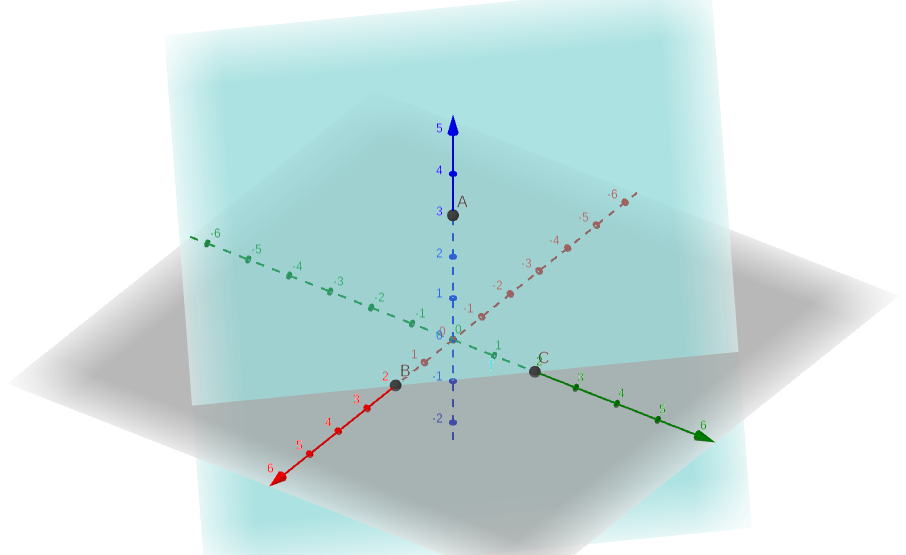
\includegraphics[scale=0.4]{../../common/img/exercises/2/1-a.png} 
\centering
\label{fig:2-1-a}
\end{figure}

\subsection*{2.1.b}
\label{subsec:2.1.b}
\addcontentsline{toc}{subsection}{\nameref{subsec:2.1.b}}

Dado que $z = \sqrt{y-x}$, para que la raíz cuadrada esté definida, debe ser $y-x \geq 0 \Rightarrow y \geq 0$. Por lo tanto:

\begin{equation}
\tcboxmath[colback=orange!25!white,colframe=orange,title=2.1.b]
{
\begin{array}{ll}
A = \mathop{Dom}(f) = \{ (x,y) \in \Bbb R^2 / y \geq x \} \\
\text{A es cerrado } (\overline{A} = A) \\
\text{A NO es abierto} (A^{\circ} \neq A) \\
\text{A NO es acotado} \\
\end{array} 
}
\end{equation}

La imagen de $f$ son cero y todos los reales positivos, por ser una raíz cuadrada. Por lo tanto, el conjunto de nivel $C_k(f)$ sólo está definido para $k \geq 0$, y consiste en:

\begin{equation}
C_k(f) = \{ (x,y) \in \Bbb R^2 / \sqrt{y-x} = k, k \in [0, +\infty) \}
\end{equation}

Despejando $y$ como función de $x$ parametrizada en $k$, resulta:

\begin{equation}
\tcboxmath[colback=orange!25!white,colframe=orange,title=2.1.b]
{
C_k(f) = \{ (x,y) \in \Bbb R^2 / y = x + k^2, k \in [0, +\infty) \}
}
\end{equation}

Así, los conjuntos de nivel son rectas de pendiente 1 desplazadas.

En cuanto al gráfico, si se piensa $z$ como una función de $y$ donde $x$ es un desplazamiento, se ve que la superficie $z$ está formada por curvas raíz cuadrada que nacen de la recta $y = x$ y crecen hacia el infinito. Véase la figura \ref{fig:2-1-b}.

\begin{figure}[ht]
\caption{\textbf{2-1-b}}
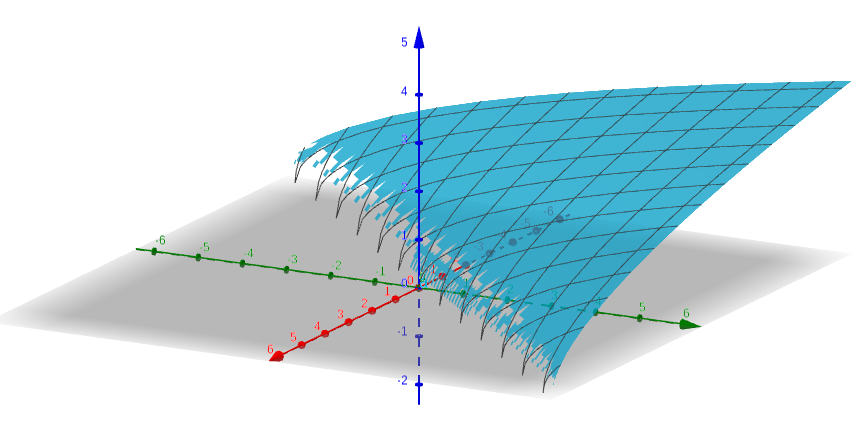
\includegraphics[scale=0.4]{../img/exercises/guide_02/01_b.png} 
\centering
\label{fig:2-1-b}
\end{figure}

\subsection*{2.1.c}
\label{subsec:2.1.c}
\addcontentsline{toc}{subsection}{\nameref{subsec:2.1.c}}

El dominio de $f$ estará dado por los valores que hagan cero o positivo el radicando: $4-x^2-y^2 \geq 0 \Leftrightarrow 4 \geq x^2 + y^2$. Ergo:

\begin{equation}
\tcboxmath[colback=orange!25!white,colframe=orange,title=2.1.c]
{
\begin{array}{ll}
A = \mathop{Dom}(f) = \{ (x,y) \in \Bbb R^2 / x^2 + y^2 \leq 4 \} \\
\text{A es cerrado } (\overline{A} = A) \\
\text{A NO es abierto } (A^{\circ} \neq A) \\
\text{A es acotado (totalmente contenido en un círculo de radio 3) } \\
\end{array} 
}
\end{equation}

Para los conjuntos de nivel, considérese primero la imagen de $f$. Su máximo valor corresponde al origen, ya que $(x,y) = (0,0)$ maximiza el radicando y por ende la raíz. En dicho caso, $z = 2$. Ahora bien, el dominio limita $x$ e $y$ de tal forma que el máximo valor que pueden tomar es $2$. En esos casos, $z = 0$. Por lo tanto, $Img(f) = [0, 2]$. Y los conjuntos de nivel resultan:

\begin{equation}
C_k(f) = \{ (x,y) \in \Bbb R^2 / \sqrt{4-x^2-y^2 = k}, 0 \leq k \leq 2 \}
\end{equation}

Estas curvas pueden expresarse como circunferencias, elevando su expresión al cuadrado miembro a miembro y acomodado:

\begin{equation}
\tcboxmath[colback=orange!25!white,colframe=orange,title=2.1.c]
{ C_k(f) = \{ (x,y) \in \Bbb R^2 / x^2+y^2 = 4-k^2, 0 \leq k \leq 2 \} }
\end{equation}

Para el gráfico, ya se saben varias cosas clave: el dominio es el interior del círculo de radio 2, $z$ varía entre 0 y 2, el máximo está en en el origen, y el mínimo en los bordes del círculo. Además, si los conjuntos de nivel son circunferencias, la superficie es una especie de cúpula circular. La figura \ref{fig:2-1-c} lo comprueba.

\begin{figure}[ht]
\caption{\textbf{2-1-c}}
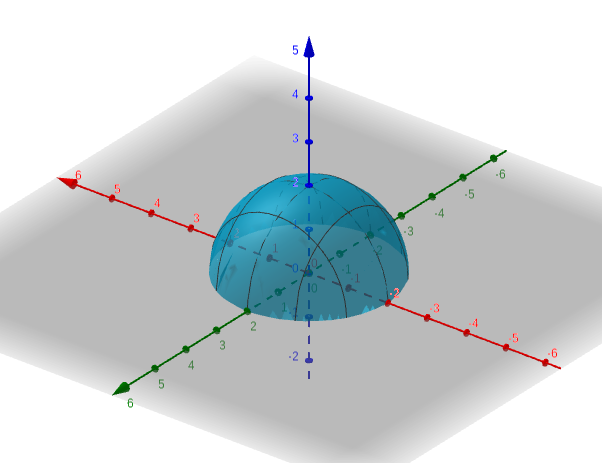
\includegraphics[scale=0.4]{../img/exercises/guide_02/01_c.png} 
\centering
\label{fig:2-1-c}
\end{figure}

\subsection*{2.1.d}
\label{subsec:2.1.d}
\addcontentsline{toc}{subsection}{\nameref{subsec:2.1.d}}

En este caso, el dominio es todo $\Bbb R^2$.

\begin{equation}
\tcboxmath[colback=orange!25!white,colframe=orange,title=2.1.d]
{
\begin{array}{ll}
A = \mathop{Dom}(f) = \Bbb R^2 \\
\text{A NO es cerrado} \\
\text{A es abierto} \\
\text{A NO es acotado} \\
\end{array} 
}
\end{equation}

En cuanto a la imagen, $z$ es la suma de dos cuadrados, por lo que sólo puede ser positivo: $\mathop{Img}(f) = [0, +\infty)$. Por lo tanto, los conjuntos de nivel serán:

\begin{equation}
C_k(f) = \{ (x,y) \in \Bbb R^2 / 9x^2 + 4 y^2 = k, k \in [0, +\infty] \}
\end{equation}

Observando fijo la expresión, corresponde a elipses cuyos semiejes crecen con $k$; y el de $x$ siempre es mayor.

\begin{equation}
\tcboxmath[colback=orange!25!white,colframe=orange,title=2.1.d]
{ C_k(f) = \left\{ (x,y) \in \Bbb R^2 / \frac{x^2}{ \left( \sqrt{\frac{k}{9}} \right)^2 } + \frac{y^2}{ \left(\sqrt{\frac{k}{4}}\right)^2 } = 1, k \in [0, +\infty] \right\} }
\end{equation}

Considerando que la imagen es $[0, +\infty)$, y los conjuntos de nivel son elipses, el gráfico de $f$ es un paraboloide elíptico, más ``estirado'' en la dirección $x$, por ser mayor ese semieje. La figura \ref{fig:2-1-d} demuestra esto.

\begin{figure}[ht]
\caption{\textbf{2-1-d}}
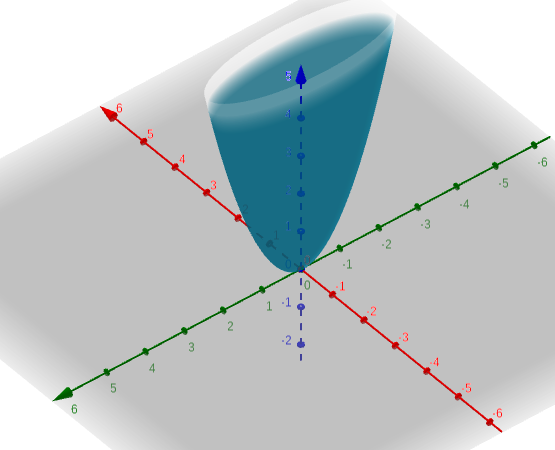
\includegraphics[scale=0.4]{../img/exercises/guide_02/01_d.png} 
\centering
\label{fig:2-1-d}
\end{figure}

\subsection*{2.1.e}
\label{subsec:2.1.e}
\addcontentsline{toc}{subsection}{\nameref{subsec:2.1.e}}

Para cualquier combinación de $x$ e $y$, $z$ está bien definido. Por ende:

\begin{equation}
\tcboxmath[colback=orange!25!white,colframe=orange,title=2.1.e]
{
\begin{array}{ll}
A = \mathop{Dom}(f) = \Bbb R^2 \\
\text{A NO es cerrado} \\
\text{A es abierto} \\
\text{A NO es acotado} \\
\end{array} 
}
\end{equation}

Considerando los conjuntos de nivel, la imagen de $f$ es todo $\Bbb R$. Y observando la expresión $x^2 - y^2 = k$, puede expresarse como hipérbolas (en tanto $k \neq 0$):

\begin{equation}
\tcboxmath[colback=orange!25!white,colframe=orange,title=2.1.e]
{ C_k(f) = \left\{ (x,y) \in \Bbb R^2 / \frac{x^2}{k} - \frac{y^2}{k} = 1, k \neq 0 \right\} }
\end{equation}

Nótese que para $k < 0$, se intercambian los signos de los sumandos, y por ende la simetría pasa del eje $y$ al $x$. 

El conjunto $C_0(f)$ corresponde a $x^2 - y^2 = 0 \Leftrightarrow x^2 = y^2 \Leftrightarrow |y| = |x|$. Para $y \geq 0$, es la curva $y = |x|$. Y para $y < 0$, es $y = -|x|$.

\begin{equation}
\tcboxmath[colback=orange!25!white,colframe=orange,title=2.1.e]
{ C_0(f) = \left\{ (x,y) \in \Bbb R^2 / y = |x| \text{ para } y \geq 0, y = -|x| \text{ para } y < 0 \right\} }
\end{equation}

Considerando que los conjuntos de nivel son las diagonales en $z = 0$, e hipérbolas de separación entre curvas creciente con $k$, el gráfico de $f$ es un paraboloide hiperbólico con punto silla en el origen. La simetría cambia para $z < 0$ como se vio al analizar $C_k(f)$. Ver figura \ref{fig:2-1-e}.

\begin{figure}[ht]
\caption{\textbf{2-1-e}}
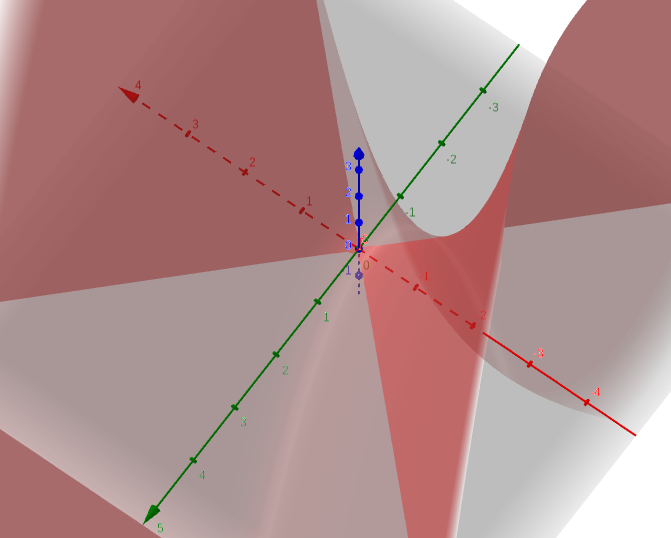
\includegraphics[scale=0.4]{../img/exercises/guide_02/01_e.png} 
\centering
\label{fig:2-1-e}
\end{figure}

\subsection*{2.1.f}
\label{subsec:2.1.f}
\addcontentsline{toc}{subsection}{\nameref{subsec:2.1.f}}

Para que $f$ esté bien definida en los reales, debe ser $16-x^2-y^2 > 0$  (el igual se quita para no dividir por cero). Entonces:

\begin{equation}
\tcboxmath[colback=orange!25!white,colframe=orange,title=2.1.f]
{
\begin{array}{ll}
A = \mathop{Dom}(f) = \{ (x,y) \in \Bbb R^2 / x^2 + y^2 < 16 \} \\
\text{A NO es cerrado} \\
\text{A es abierto} \\
\text{A es acotado} \\
\end{array} 
}
\end{equation}

La imagen de $f$ tiene su minímo en el origen, porque se maximiza el numerador. En dicho caso, $z = \frac{1}{4}$. A medida que los puntos se acercan al círculo de radio 4, el numerador se acerca a $0^+$, y por ende $z$ tiende a $+\infty$. Los conjuntos de nivel son entonces:

\begin{equation}
C_k(f) = \{ (x,y) \in \Bbb R^2 / \frac{1}{\sqrt{16-x^2-y^2}} = k, k \geq \frac{1}{4} \}
\end{equation}

Elevando al cuadrado miembro a miembro y acomodando, los $C_k$ resultan circunferencias:

\begin{equation}
\tcboxmath[colback=orange!25!white,colframe=orange,title=2.1.e]
{ C_k(f) = \{ (x,y) \in \Bbb R^2 / x^2 + y^2 = 16 -\frac{1}{k^2}, k \geq \frac{1}{4} \} }
\end{equation}

Considerando los conjuntos de nivel, el gráfico comienza en $z = \frac{1}{4}$, donde es sólo un punto. Para mayor $z$, son circunferencias que tienden rápidamente hacia la circunferencia de radio 4, pero jamás la alcanzan porque hay un infinitésimo restando. Por lo tanto, la superficie de $z=f(x,y)$ tiene forma de paraboloide; tiene su mínimo en $(0, 0, \frac{1}{4})$ y crece hacia infinito positivo, pero sin salirse del cilindro de radio $4$. La figura \ref{fig:2-1-f} corrobora esto.

\begin{figure}[ht]
\caption{\textbf{2.1.f}}
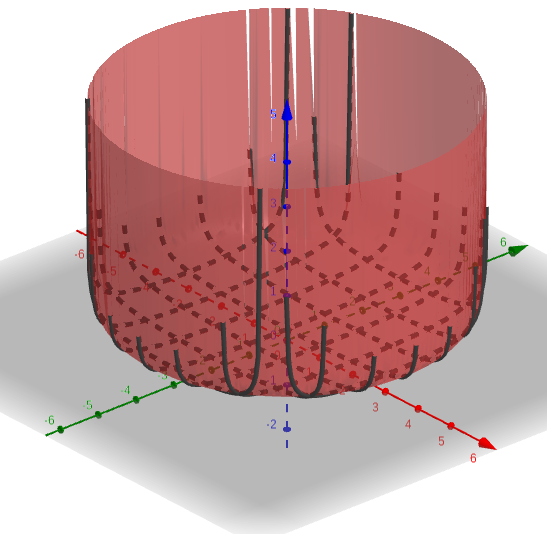
\includegraphics[scale=0.4]{../img/exercises/guide_02/01_f.png} 
\centering
\label{fig:2-1-f}
\end{figure}

\subsection*{2.1.g}
\label{subsec:2.1.g}
\addcontentsline{toc}{subsection}{\nameref{subsec:2.1.g}}

La función $f$ está definida para todo valor; por lo tanto,

\begin{equation}
\tcboxmath[colback=orange!25!white,colframe=orange,title=2.1.g]
{
\begin{array}{ll}
A = \mathop{Dom}(f) = \Bbb R^2 \\
\text{A NO es cerrado} \\
\text{A es abierto} \\
\text{A NO es acotado} \\
\end{array} 
}
\end{equation}

La imagen es $(-\infty, 25]$, ya que el valor mínimo que puede tomar $-x^2$ es cero. Por ende, los conjuntos de nivel son:

\begin{equation}
C_k(f) = \{ (x,y) \in \Bbb R^2 / 25-x^2 = k, k \leq 25 \}
\end{equation}

Despejando $x$, resulta: 

\begin{equation}
\tcboxmath[colback=orange!25!white,colframe=orange,title=2.1.g]
{ C_k(f) = \{ (x,y) \in \Bbb R^2 / x = \pm \sqrt{25-k}, k \leq 25 \} }
\end{equation}

Ergo, los conjuntos de nivel son pares de rectas paralelas y equidistantes al eje $x$. Para visualizar el gráfico, considérese que $y$ es una variable libre. La curva que ocurra en el plano $y = 0$ será idéntica para cualquier otro valor de $y$. Por lo tanto, observando el plano $xz$ en $y=0$, se tiene una simple parábola invertida, que alcanza su máximo en $x=0, z=25$, y corta al eje $x$ en $x=\pm5$. Replicando esa curva a lo largo del eje $y$, se obtiene la superficie de la figura \ref{fig:2-1-g}.

\begin{figure}[ht]
\caption{\textbf{2.1.g}}
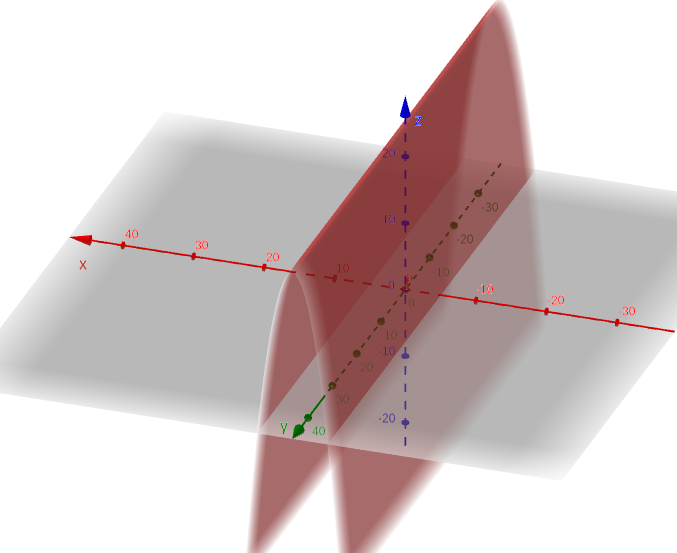
\includegraphics[scale=0.4]{../img/exercises/guide_02/01_g.png} 
\centering
\label{fig:2-1-g}
\end{figure}

\subsection*{2.1.h}
\label{subsec:2.1.h}
\addcontentsline{toc}{subsection}{\nameref{subsec:2.1.h}}

La función $f(x,y)$ está definida para toda combinación de $x$ e $y$. Ergo:

\begin{equation}
\tcboxmath[colback=orange!25!white,colframe=orange,title=2.1.h]
{
\begin{array}{ll}
A = \mathop{Dom}(f) = \Bbb R^2 \\
\text{A NO es cerrado} \\
\text{A es abierto} \\
\text{A NO es acotado} \\
\end{array} 
}
\end{equation}

La imagen de $f$ corresponde a una exponencial real cuyo exponente siempre es cero o negativo (por los cuadrados negados). Por lo tanto, el máximo valor que puede tomar es 1, en el origen. Para otros valores, tenderá a cero. Por ende, $\mathop{Img}(f) = (0, 1]$. Y los conjuntos de nivel están dados por:

\begin{equation}
C_k(f) = \{ (x,y) \in \Bbb R^2 / e^{-x^2-y^2} = k, 0 < k \leq 1 \}
\end{equation}

Aplicando la función $\ln$ miembro a miembro y acomodando, se ve que estas curvas son circunferencias.

\begin{equation}
\tcboxmath[colback=orange!25!white,colframe=orange,title=2.1.h]
{ C_k(f) = \left\{ (x,y) \in \Bbb R^2 / x^2+y^2 = \ln \left( \frac{1}{k} \right), 0 < k \leq 1 \right\} }
\end{equation}

Considerando la imagen y los conjuntos de nivel, el gráfico de $f$ debería ser como una campana de Gauss en las direcciones de $x$ e $y$, con su máximo en el origen y tendiendo a cero de forma rápida pero suave. La figura \ref{fig:2-1-h} corrobora esto.

\begin{figure}[ht]
\caption{\textbf{2.1.h}}
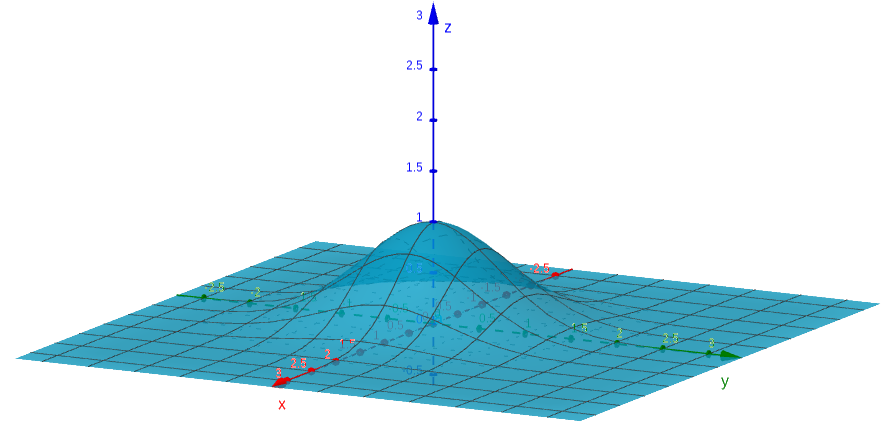
\includegraphics[scale=0.4]{../img/exercises/guide_02/01_h.png} 
\centering
\label{fig:2-1-h}
\end{figure}

\subsection*{2.1.i}
\label{subsec:2.1.i}
\addcontentsline{toc}{subsection}{\nameref{subsec:2.1.i}}

El radicando eleva $x$ e $y$ al cuadrado, lo cual impide que sea negativo. Por lo tanto, $f$ está definida para todo $\Bbb R^2$.

\begin{equation}
\tcboxmath[colback=orange!25!white,colframe=orange,title=2.1.i]
{
\begin{array}{ll}
A = \mathop{Dom}(f) = \Bbb R^2 \\
\text{A NO es cerrado} \\
\text{A es abierto} \\
\text{A NO es acotado} \\
\end{array} 
}
\end{equation}

La imagen de $f$ tiene que ser cero o positiva por ser una raíz cuadrada de valores entre 0 y $+\infty$: $Im(f) = [0, +\infty]$. Los conjuntos de nivel resultan entonces:

\begin{equation}
C_k(f) = \{ (x,y) \in \Bbb R^2 / \sqrt{x^2 + 2y^2} = k, k \geq 0 \}
\end{equation}

Elevando al cuadrado miembro a miembro, se ve que estas curvas son elipses. Acomodando para reflejar eso:

\begin{equation}
\tcboxmath[colback=orange!25!white,colframe=orange,title=2.1.i]
{
\begin{array}{ll}
C_k(f) = \left\{ (x,y) \in \Bbb R^2 / \frac{x^2}{k^2} + \frac{y^2}{\frac{k^2}{2}} = 1, k > 0 \right\} \\
C_0(f) = (0, 0)
\end{array}
}
\end{equation}

Considerando la imagen y conjuntos de nivel, el gráfico debería ser una especie de paraboloide elíptico, cuyo mínimo está en el origen, y crece hacia infinito. El ancho en $x$ será siempre el doble que en $y$, por las relaciones entre los semiejes. La figura \ref{fig:2-1-i} confirma esto, con un agregado: los radios de las elipses crecen linealmente con $z$; visualmente, la superficie es más un cono que un paraboloide. Esto tiene sentido observando que en $C_k(f)$, $k$ está elevado al cuadrado, igual que $x$ e $y$.

\begin{figure}[ht]
\caption{\textbf{2.1.i}}
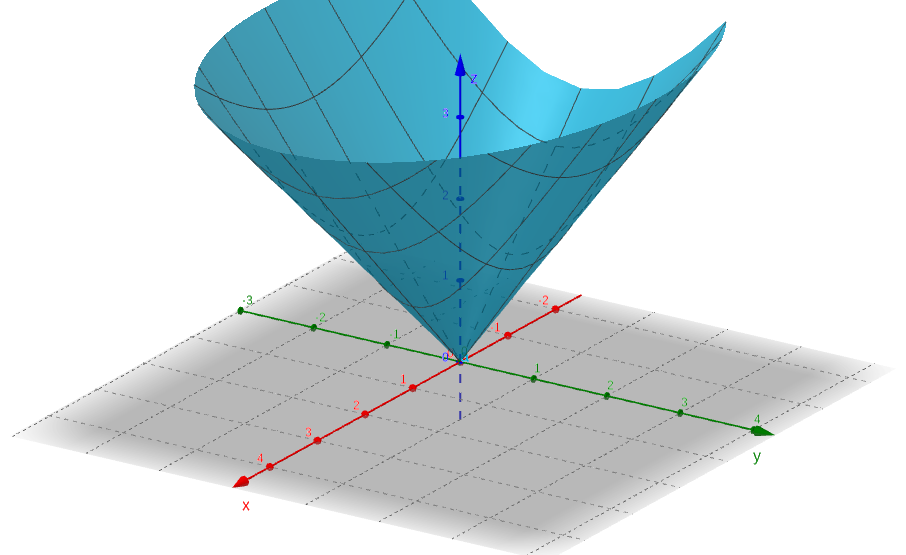
\includegraphics[scale=0.4]{../img/exercises/guide_02/01_i.png} 
\centering
\label{fig:2-1-i}
\end{figure}

\subsection*{2.1.j}
\label{subsec:2.1.j}
\addcontentsline{toc}{subsection}{\nameref{subsec:2.1.j}}

No hay ninguna combinación de $x$ e $y$ que cause alguna indeterminación; $f$ siempre está bien definida. Por lo tanto:

\begin{equation}
\tcboxmath[colback=orange!25!white,colframe=orange,title=2.1.j]
{
\begin{array}{ll}
A = \mathop{Dom}(f) = \Bbb R^2 \\
\text{A NO es cerrado} \\
\text{A es abierto} \\
\text{A NO es acotado} \\
\end{array} 
}
\end{equation}

La imagen es claramente todo $\Bbb R$, ya que $x$ e $y$ pueden tomar cualquier valor. En cuanto a los conjuntos de nivel, su planteo por definición sería:

\begin{equation}
C_k(f) = \{ (x,y) \in \Bbb R^2 / \min(x,y) = k, k \in \Bbb R \}
\end{equation}

Para cada valor fijo $k$, hay 3 puntos que satisfacen la igualdad:

\begin{equation}
\begin{array}{ll}
(k, k, k) \text{ si } x = y \\
(x, k, k) \text{ si } y < x \\
(k, y, k) \text{ si } x < y
\end{array}
\end{equation}

Por lo tanto, cada conjunto de nivel es un trío de puntos:

\begin{equation}
\tcboxmath[colback=orange!25!white,colframe=orange,title=2.1.j]
{ C_k(f) = \{ (x,y) \in \Bbb R^2 / (x,y)=(k,k) \vee (x,y)=(x,k) \vee (x,y)=(k,y), k \in \Bbb R \} }
\end{equation}

Para el gráfico, en esta ocasión los conjuntos de nivel no ayudan mucho. Considérese el plano dominio, $xy$; el valor que toma $z = f(x,y)$ está divido por la recta $y=x$. En la región de $\Bbb R^2$ donde $y <= x$, $z = y$, y para $y < x$, $z = x$. Ergo, $f$ puede expresarse de la siguiente manera:

\begin{equation}
z = f(x,y) = \left\{ \begin{array}{ll}
y \text{ si } y \leq x \\
x \text{ si } y > x
\end{array} \right.
\end{equation}

Ambas ramas de $f$ pueden considerarse como planos. Más concretamente, el plano $z = y$ es la recta $z = y$ en el plano $zy$, replicada a lo largo del eje $x$. Análogamente, el plano $z = x$ es la recta $z = x$ replicada a lo largo del eje $y$. Con esto en mente, el gráfico de $f$ se construye tomando las secciones de ambos planos correspondientes a cada región, y considerando que los planos se intersectan en la recta $y = x$. Esto es consistente con que los conjuntos de nivel sean tríos de puntos: un punto en el plano $z = y$, otro en el plano $z = x$, y otro sobre la recta donde se cortan los planos.

\begin{figure}[ht]
\caption{\textbf{2.1.j}}
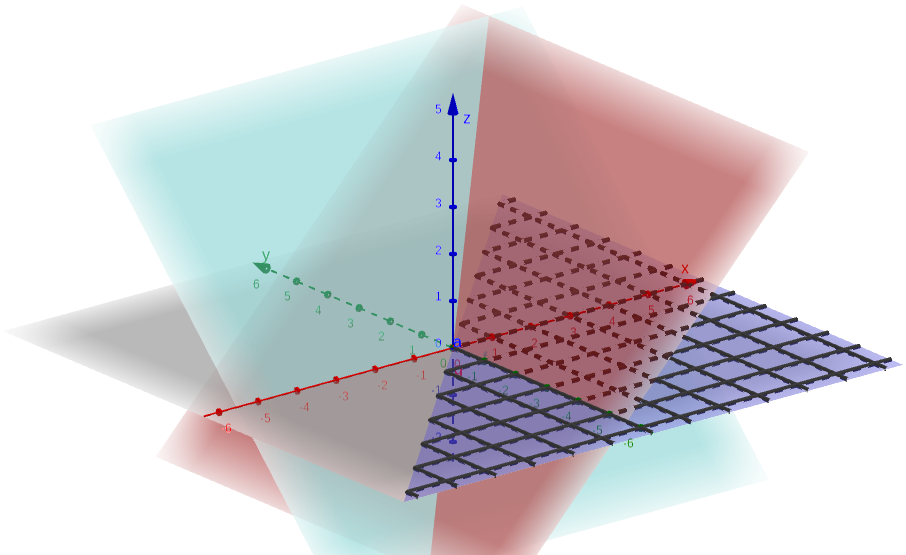
\includegraphics[scale=0.4]{../img/exercises/guide_02/01_j.png} 
\centering
\label{fig:2-1-j}
\end{figure}

En la figura \ref{fig:2-1-j}, el plano $z = y$ se halla graficado en color cian, y el plano $z = x$ en rojo. La región $y \leq x$ en el plano $z = 0$ se halla marcada con una grilla a modo de referencia. Gracias a dicha referencia, es sencillo ver que el gráfico de $f$ corresponde a las mitades ``decrecientes'' de los planos demarcados por la recta $y = x$ y su proyección. Burdamente, el gráfico de $f$ es como un techo a dos aguas.

\subsection*{2.1.k}
\label{subsec:2.1.k}
\addcontentsline{toc}{subsection}{\nameref{subsec:2.1.k}}

Aplicando el mismo razonamiento que en el inciso anterior, con la única diferencia de tomar el máximo en lugar del mínimo:

\begin{equation}
\tcboxmath[colback=orange!25!white,colframe=orange,title=2.1.k]
{
\begin{array}{ll}
A = \mathop{Dom}(f) = \Bbb R^2 \\
\text{A NO es cerrado} \\
\text{A es abierto} \\
\text{A NO es acotado} \\
\end{array} 
}
\end{equation}

\begin{equation}
\tcboxmath[colback=orange!25!white,colframe=orange,title=2.1.j]
{ C_k(f) = \{ (x,y) \in \Bbb R^2 / (x,y)=(k,k) \vee (x,y)=(x,k) \vee (x,y)=(k,y), k \in \Bbb R \} }
\end{equation}

La definición por partes de $f$ intercambia los semiplanos:

\begin{equation}
z = f(x,y) = \left\{ \begin{array}{ll}
x \text{ si } y \leq x \\
y \text{ si } y > x
\end{array} \right.
\end{equation}

Por lo tanto, tomando como referencia la figura \ref{fig:2-1-j}, el gráfico de $f$ corresponde a las secciones ``crecientes'' de los planos $z = x$ y $z = y$. Es un techo a dos aguas invertido.

\hrule
\vspace{10 pt}

\section*{2.2}
\label{sec:2.2}
\addcontentsline{toc}{section}{\nameref{sec:2.2}}

\textbf{En los siguientes casos hallar, si existe, el límite indicado; en los casos en que no existe, fundamentar.} 

\begin{enumerate}[(a)]
\bfseries
\item $ \lim_{(x,y) \rightarrow (1,-1)} xy - y^2 $
\item $ \lim_{(x,y) \rightarrow (0,0)} \frac{x^2 + y^2}{y} $
\item $ \lim_{(x,y) \rightarrow (0,0)} \sqrt{x^2 + y^2} $
\item $ \lim_{(x,y) \rightarrow (1,-2)} x^2 + (y-2)^2 x $
\item $ \lim_{(x,y) \rightarrow (0,2)} \frac{y^2 (x-2)^2}{x^2 + (y-2)^2} $
\item $ \lim_{(x,y) \rightarrow (0,4)} \frac{x}{\sqrt{y}} $
\item $ \lim_{(x,y) \rightarrow (1,-2)} \left( xy, \frac{y}{x+1}, \sqrt{x^2 + y^2} \right) $
\item $ \lim_{(x,y,z) \rightarrow (0,1,1)} \frac{y+1}{\sqrt{z^2 - 1}} $
\item $ \lim_{(x,y) \rightarrow (0,0)} \left( y \cos\left(\frac{1}{x}\right), \frac{\sin(3x)}{2x}, x-y \right) $
\end{enumerate}
\hrule

\subsection*{2.2.a}
\label{subsec:2.2.a}
\addcontentsline{toc}{subsection}{\nameref{subsec:2.2.a}}

La función $f(x,y) = xy - x^2$ es continua en todo $\Bbb R^2$. Por lo tanto:

\begin{equation}
\tcboxmath[colback=orange!25!white,colframe=orange,title=2.2.a]
{ \lim_{(x,y) \rightarrow (1,-1)} f(x,y) = f(1,-1) = -2 }
\end{equation}

\subsection*{2.2.b}
\label{subsec:2.2.b}
\addcontentsline{toc}{subsection}{\nameref{subsec:2.2.b}}

Esta función tiene una singularidad en $(0, 0)$. Probando con los límites sucesivos:

\begin{align}
l_{12} = \lim_{y \rightarrow 0} \left( \lim_{x \rightarrow 0} \frac{x^2 + y^2}{y} \right) = \lim_{y \rightarrow 0} y = 0 \\
l_{21} = \lim_{x \rightarrow 0} \left( \lim_{y \rightarrow 0} \frac{x^2 + y^2}{y} \right) = \lim_{x \rightarrow 0} \infty
\end{align}

Si el límite existe, tiene que ser único. Por lo tanto, que difieran los límites sucesivos garantiza que:

\begin{equation}
\tcboxmath[colback=orange!25!white,colframe=orange,title=2.2.b]
{ \lim_{(x,y) \rightarrow (0,0)} \frac{x^2 + y^2}{y} = \nexists }
\end{equation}

\subsection*{2.2.c}
\label{subsec:2.2.c}
\addcontentsline{toc}{subsection}{\nameref{subsec:2.2.c}}

No hay singularidades en $f$.

\begin{equation}
\tcboxmath[colback=orange!25!white,colframe=orange,title=2.2.c]
{ \lim_{(x,y) \rightarrow (0,0)} \sqrt{x^2 + y^2} = 0 }
\end{equation}

\subsection*{2.2.d}
\label{subsec:2.2.d}
\addcontentsline{toc}{subsection}{\nameref{subsec:2.2.d}}

No hay singularidades en $f$.

\begin{equation}
\tcboxmath[colback=orange!25!white,colframe=orange,title=2.2.d]
{ \lim_{(x,y) \rightarrow (1,-2)} x^2 + (y-2)^2 x = 5 }
\end{equation}

\subsection*{2.2.e}
\label{subsec:2.2.e}
\addcontentsline{toc}{subsection}{\nameref{subsec:2.2.e}}

Evaluando el límite de forma directa, se ve que la función $f$ tiende a $+\infty$ cuando $(x,y)$ tiende a $(0,2)$. Por definición, si el límite existe, es un número real finito, o un vector con todas sus componentes reales y finitas. Por lo tanto, se puede concluir el ejercicio diciendo que el límite no existe.

\begin{equation}
\tcboxmath[colback=orange!25!white,colframe=orange,title=2.2.e]
{ \lim_{(x,y) \rightarrow (0,2)} \frac{y^2 (x-2)^2}{x^2 + (y-2)^2} = \frac{16}{0^+} = +\infty = \nexists }
\end{equation}

En un análisis más detallado, se puede afirmar que al ser todos los sumandos y factores cuadrados, $f$ sólo toma valores positivos, por ende es imposible que haya una forma de aproximarse a $(0,2)$ que haga tender a $f$ a $-\infty$. Tal vez exista una forma de hacerlo finito, pero eso no cambiará el hecho de que el límite no existe. 

\subsection*{2.2.f}
\label{subsec:2.2.f}
\addcontentsline{toc}{subsection}{\nameref{subsec:2.2.f}}

La función $f$ es continua en el punto de interés, $(0, 4)$. Sus infinitas singularidades están sobre la recta $y = 0$. Por lo tanto, el límite existe y vale:

\begin{equation}
\tcboxmath[colback=orange!25!white,colframe=orange,title=2.2.f]
{ \lim_{(x,y) \rightarrow (0,4)} \frac{x}{\sqrt{y}} = \frac{0}{2} = 0 }
\end{equation}

\subsection*{2.2.g}
\label{subsec:2.2.g}
\addcontentsline{toc}{subsection}{\nameref{subsec:2.2.g}}

El límite de un campo vectorial es el vector formado por los límites de los campos escalares componentes, si y sólo si todos esos límites existen. En este caso particular, el campo vectorial es:

\begin{equation}
f: \Bbb R^2 \rightarrow \Bbb R^3 / f(x,y) = \left( x y, \frac{y}{x+1}, \sqrt{x^2 + y^2} \right)
\end{equation}

El primer y tercer campo escalar están bien definidos para todo par $(x,y)$. En cambio, el segundo tiene infinitas singularidades, sobre la recta $x = -1$. En todo otro punto, $f$ es continua. El punto del límite es uno de estos últimos. En consecuencia:

\begin{equation}
\tcboxmath[colback=orange!25!white,colframe=orange,title=2.2.g]
{ \lim_{(x,y) \rightarrow (1,-2)} f(x,y) = f(1,-2) = (-2, -1, \sqrt{5}) }
\end{equation}

\subsection*{2.2.h}
\label{subsec:2.2.h}
\addcontentsline{toc}{subsection}{\nameref{subsec:2.2.h}}

De forma similar a 2.2.e, al evaluar el límite de forma directa, el mismo resulta infinito. Por lo tanto, se puede concluir que el límite no existe.

\begin{equation}
\tcboxmath[colback=orange!25!white,colframe=orange,title=2.2.h]
{ \lim_{(x,y,z) \rightarrow (0,1,1)} \frac{y+1}{\sqrt{z^2-1}} = \frac{2}{0} = \infty = \nexists }
\end{equation}

El denominador siempre es positivo, pero el numerador puede cambiar de signo. Según $y$ tienda a $1$ por derecha o izquierda, $f$ tenderá a infinito positivo o negativo.

\subsection*{2.2.i}
\label{subsec:2.2.i}
\addcontentsline{toc}{subsection}{\nameref{subsec:2.2.i}}

Nuevamente, al tener un campo vectorial, hay que analizar por separado sus componentes.
Para el primero, la propiedad de cero por acotado sigue valiendo para $n$ variables.

\begin{equation}
\lim_{(x,y) \rightarrow (0,0)} \underbrace{y}_{\rightarrow 0} \underbrace{ \cos \left( \frac{1}{x} \right) }_{\in [-1,1] \forall x} = 0
\end{equation}

En el segundo caso, es un límite de una sola variable. Es válido aplicar la regla de L'Hôpital.

\begin{equation}
\lim_{(x,y) \rightarrow (0,0)} \frac{\sin (3x)}{2x} = \lim_{x \rightarrow 0} \frac{\sin (3x)}{2x} = \lim_{x \rightarrow 0} \frac{3 \cos(3x)}{2} = \frac{3}{2}
\end{equation}

El tercer campo escalar es continuo en todo $\Bbb R^2$, su límite existe y es trivial. Por ende, dado que todos los campos escalares componentes tienen límite bien definido, el límite del campo vectorial que componen está bien definido.

\begin{equation}
\tcboxmath[colback=orange!25!white,colframe=orange,title=2.2.i]
{ \lim_{(x,y) \rightarrow (0,0) } \overline{f}(x,y) = \left( 0, \frac{3}{2}, 0 \right) }
\end{equation}

\hrule
\vspace{10 pt}

\section*{2.3}
\label{sec:2.3}
\addcontentsline{toc}{section}{\nameref{sec:2.3}}

\textbf{En los siguientes casos hallar, cuando sea posible hallar una función que satisfaga las condiciones dadas. Si ello no es posible, fundamentar.} 

\begin{enumerate}[(a)]
\bfseries
\item $ f(x,y) > 0$ cuando $x > 0 \wedge y > 0$, $\lim_{(x,y) \rightarrow (0,0)} f(x,y) = 0$

\item $f(x,y) > 1$ cuando $y > x^2 + 1$, $f(x,y) < 1$ cuando $y < x^2 + 1$, y $\lim_{(x,y) \rightarrow (0,1)} f(x,y) = 1$
\end{enumerate}
\hrule

\subsection*{2.3.a}
\label{subsec:2.3.a}
\addcontentsline{toc}{subsection}{\nameref{subsec:2.3.a}}

Una función que es positiva en el primer cuadrante y tiende a cero en el origen es:

\begin{equation}
\tcboxmath[colback=orange!25!white,colframe=orange,title=2.3.a]
{ f(x,y) = x + y }
\end{equation}

\subsection*{2.3.b}
\label{subsec:2.3.b}
\addcontentsline{toc}{subsection}{\nameref{subsec:2.3.b}}

Manipulando las condiciones:

\begin{align}
y > x^2 + 1 \Rightarrow \frac{y}{x^2 + 1} > 1 \\
y < x^2 + 1 \Rightarrow \frac{y}{x^2 + 1} < 1
\end{align}

Esto sugiere la conveniencia de definir $f(x,y) = \frac{y}{x^2+1}$. Si satisface el límite pedido, es una solución válida.
Por continuidad de $f$ en el punto $(0, 1)$:

\begin{equation}
\lim_{(x,y) \rightarrow (0,1)} \frac{y}{x^2 + 1} = \frac{1}{0+1} = 1
\end{equation}

Finalmente:

\begin{equation}
\tcboxmath[colback=orange!25!white,colframe=orange,title=2.3.b]
{ f(x,y) = \frac{y}{x^2 + 1} }
\end{equation}

\section*{2.4}
\label{sec:2.4}
\addcontentsline{toc}{section}{\nameref{sec:2.4}}

\textbf{Resolver:} 

\begin{enumerate}[(a)]
\bfseries
\item Sea $f(x,y) = \frac{x^2 + y^2 -4}{x^2 - y^2}$. Describir el dominio de $f$. Describir la región $R$ donde $f$ es positiva en coordenadas cartesianas y polares, aclarando si es o no abierta y si es o no acotada. Suponga que se define una nueva función $\hat{f}$ que coincide con $f$ en los puntos de su dominio y vale 1 en el resto del plano, es decir:

\begin{equation}
\hat{f}(x,y) = \left\{ \begin{array}{ll}
f(x,y) &\text{ si } (x,y) \in \mathop{Dom}(f) \\
1 & \text{ si } (x,y) \notin \mathop{Dom}(f)
\end{array}
\right.
\end{equation}

Analizar la continuidad de $\hat{f}$ en $(\sqrt{2}, -\sqrt{2})$.

\item Sea

\begin{equation}
f(x,y) = \left\{ \begin{array}{ll}
(1 + |2x+y|) (x^2 + y^2 -1) &\text{ si } y > x \\
x^2 + y^2 - 1 & \text{ si } y \leq x
\end{array}
\right.
\end{equation}

Describir la región $R$ donde $f$ es positiva ($> 0$) en coordenadas cartesianas y polares, aclrando si es o no abierta y si es o no acotada. Analizar la continuidad de $f$ en cada punto de la recta de ecuación $y = x$.

\item Supongamos que $f: \Bbb R^2 \rightarrow \Bbb R$ es una función de la que se sabe que es continua en todos los puntos del plano, y que es positiva ($> 0$) en la región descripta en polares por $(0 < \rho < 2) \wedge (0 < \phi < \frac{\pi}{3})$, negativa en la región descripta por $(\rho > 2) \vee (\frac{\pi}{3} < \phi < 2\pi)$ (donde $\wedge$ y $\vee$ denotan el y el o lógicos respectivamente)y $f(0,0) = 0$. Sea $g(x,y) = \frac{1}{f(y,x)}$. Describir el conjunto donde $g$ es positiva ($>0$), y analizar en qué puntos del plano $g$ es continua.

\end{enumerate}
\hrule

\subsection*{2.4.a}
\label{subsec:2.4.a}
\addcontentsline{toc}{subsection}{\nameref{subsec:2.4.a}}

En primer lugar, el dominio de $f$ es todo $\Bbb R^2$, excluyendo los ceros del denominador.

\begin{equation}
x^2 - y^2 = 0 \Leftrightarrow |x| = |y| \Leftrightarrow y = \left\{
\begin{array}{ll}
|x| \text{ si } y \geq 0 \\
-|x| \text{ si } y < 0
\end{array}
\right.
\end{equation}

\begin{equation}
\tcboxmath[colback=orange!25!white,colframe=orange,title=2.4.a. Dominio]
{ \mathop{Dom}(f) = \Bbb R^2 - \{ (x,y) \in \Bbb R^2 / |y| = |x| \} }
\end{equation}

En segundo lugar, para que $f$ sea positiva, o bien numerador y denominador son ambos positivos, o ambos negativos. Simbólicamente:

\begin{subequations}
\begin{align}
R &= \{ (x,y) \in \Bbb R^2 / f(x,y) > 0 \} = \\
& \{ (x,y) \in \Bbb R^2 / (x^2 + y^2 - 4 > 0) \wedge x^2 - y^2 > 0) \vee (x^2 + y^2 - 4 < 0 \wedge x^2 - y^2 < 0) \}
\end{align}
\end{subequations}

Resulta entonces $R$ en coordenadas cartesianas:

\begin{equation}
\tcboxmath[colback=orange!25!white,colframe=orange,title=2.4.a. R en cartesianas]
{ R = \{ (x,y) \in \Bbb R^2 / (x^2 + y^2 > 4 \wedge |x| > |y|) \vee (x^2 + y^2 < 4 \wedge |x| < |y|) \} }
\end{equation}

Graficando los dos operandos del $\vee$ por separado, se tienen las regiones de la figura \ref{fig:2-4-a}. La región azul corresponde al primer operando, y la roja al segundo. La región $R$ es la unión de ambas regiones. 

\begin{figure}[ht]
\caption{\textbf{2.4.a}}
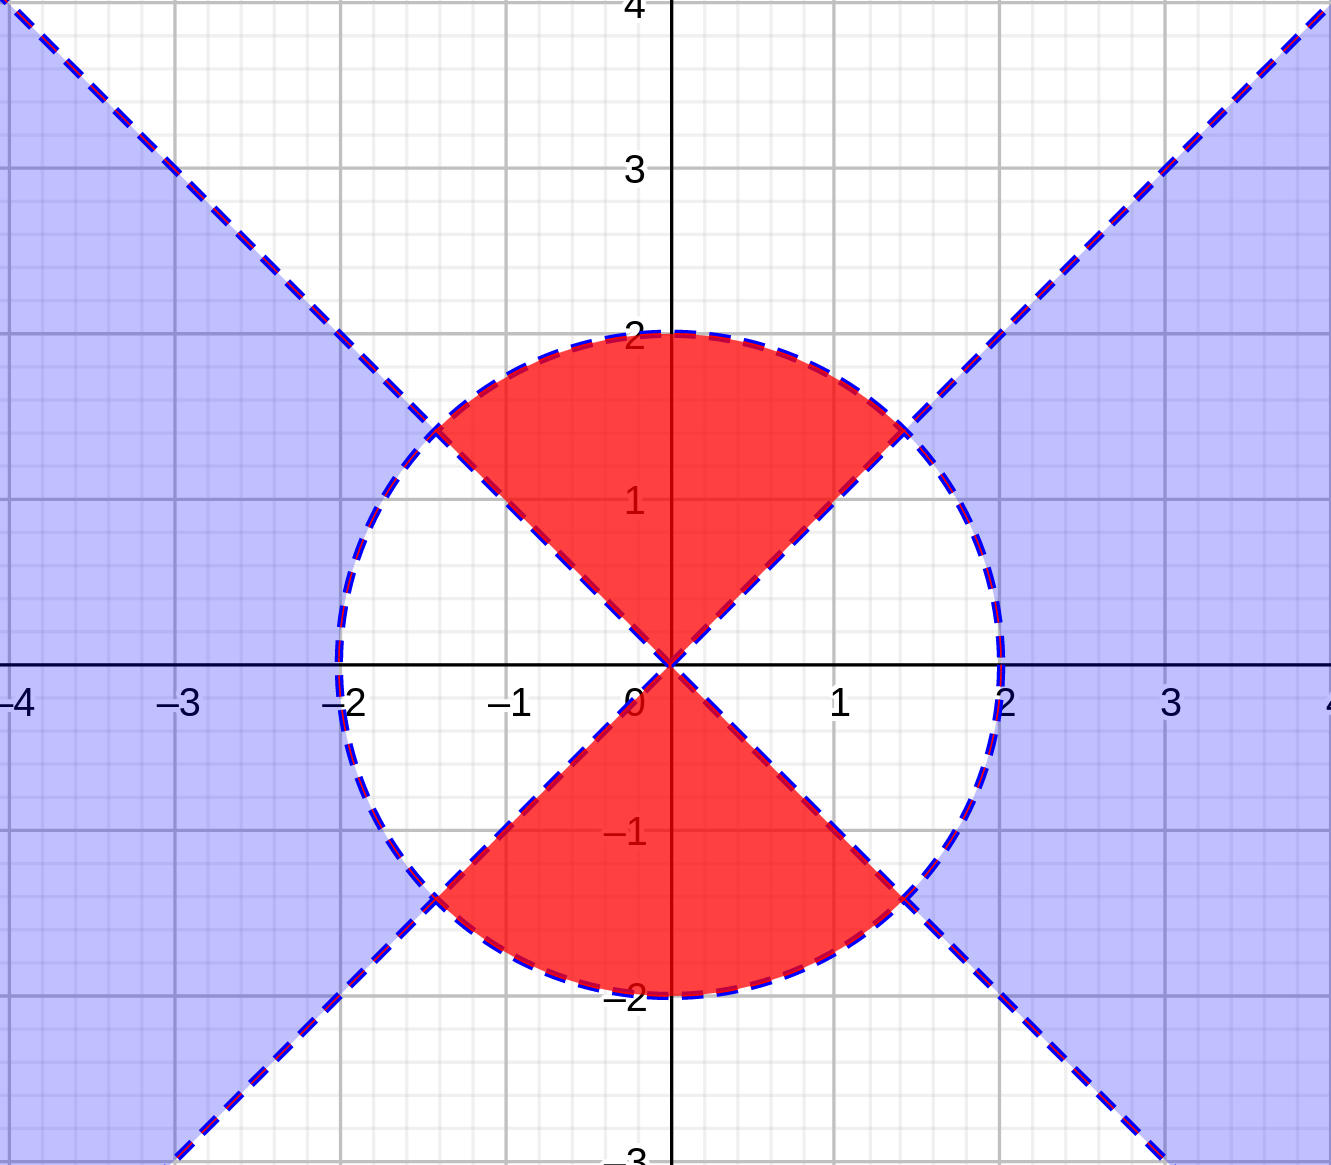
\includegraphics[scale=0.8]{../img/exercises/guide_02/04_a.png} 
\centering
\label{fig:2-4-a}
\end{figure}

En coordenadas polares:

\begin{equation}
\tcboxmath[colback=orange!25!white,colframe=orange,title=2.4.a. R en polares]
{
\begin{array}{ll}
R = &\left\{ (\rho, \phi) \in \Bbb R^2 / \left[ \rho > 2 \wedge \left( -\frac{\pi}{4} < \phi < \frac{\pi}{4} \vee \frac{3}{4}\pi < \phi < \frac{5}{4}\pi \right) \right] \vee \right. \\
& \left. [\rho < 2 \wedge \left( \frac{\pi}{4} < \phi < \frac{3}{4}\pi \vee \frac{5}{4}\pi < \phi < \frac{7}{4}\pi \right)] \right\}
\end{array}
}
\end{equation}

La región $R$ es entonces abierta y no acotada.

Para que la función $\hat{f}$ sea continua en el punto de interés, necesariamente debe cumplirse $\lim_{(x,y) \rightarrow (\sqrt{2}, -\sqrt{2})} \hat{f}(x,y) = 1$. Dado que se está evaluando el límite, $x$ e $y$ nunca llegan al valor del punto, y por ende la expresión a evaluar es la de la $f$ original. Ello conduce a la indeterminación $\frac{0}{0}$. Observando el denominador, en particular que aparece $-y^2$, se intuye que los límites iterados pueden diferer y por ende el límite no existir. Se procede a verificar dicha hipótesis:

\begin{subequations}
\begin{align}
l_{12} = \lim_{y \rightarrow -\sqrt{2}} \left( \lim_{x \rightarrow \sqrt{2}} \frac{x^2 + y^2 - 4}{x^2 - y^2} \right) = \lim_{y \rightarrow -\sqrt{2}} \frac{y^2 - 2}{-y^2 + 2} = \lim_{y \rightarrow -\sqrt{2}} \frac{2y}{-2y} = -1 \\
l_{21} = \lim_{x \rightarrow \sqrt{2}} \left( \lim_{y \rightarrow -\sqrt{2}} \frac{x^2 + y^2 - 4}{x^2 - y^2} \right) = \lim_{x \rightarrow \sqrt{2}} \frac{x^2 - 2}{x^2 + 2} = 1
\end{align}
\end{subequations}

Dado que los límites iterados difieren:

\begin{equation}
\tcboxmath[colback=orange!25!white,colframe=orange,title=2.4.a. Continuidad]
{ \hat{f}(x,y) \text{ no es continua en } (\sqrt{2}, -\sqrt{2}) }
\end{equation}

\subsection*{2.4.b}
\label{subsec:2.4.b}
\addcontentsline{toc}{subsection}{\nameref{subsec:2.4.b}}

\begin{equation}
f(x,y) = \left\{ \begin{array}{ll}
(1 + |2x + y|) (x^2 + y^2 - 1) &\text{ si } y > x \\
x^2 + y^2 - 1 &\text{ si } y \leq x
\end{array} \right.
\end{equation}

En la rama I ($y > x$), para que sea positiva, hay que analizar los signos de los factores del producto. O ambos son positivos, o ambos negativos.

\begin{itemize}
\item Ambos positivos:
	\begin{itemize}
		\item $1 + |2x + y| > 0 \Leftrightarrow |2x + y| > -1$, lo cual se cumple $\forall (x,y)$
		\item $x^2 + y^2 -1 > 0 \Leftrightarrow x^2 + y^2 > 1$
	\end{itemize}
\item Ambos negativos:
	\begin{itemize}
		\item $1 + |2x + y| < 0 \Leftrightarrow |2x + y| < -1$, lo cual por definición de valor absoluto es imposible.
	\end{itemize}
\end{itemize}

En la rama II ($y \leq x$), el análisis es más directo: $x^2 + y^2 - 1 > 0 \Leftrightarrow x^2 + y^2 > 1$. Combinando lo obtenido para las dos ramas, resulta:

\begin{equation}
\tcboxmath[colback=orange!25!white,colframe=orange,title=2.4.b. R en cartesianas]
{ R = \{ (x, y) \in \Bbb R^2 / (x^2 + y^2 > 1 \wedge y > x) \vee (x^2 + y^2 \geq 1 \wedge y \leq x) \} }
\end{equation}

Convirtiendo a polares:

\begin{equation}
\tcboxmath[colback=orange!25!white,colframe=orange,title=2.4.a. R en polares]
{
\begin{array}{ll}
R = &\left\{ (\rho, \phi) \in \Bbb R^2 / \left[ \rho > 1 \wedge \left( \frac{\pi}{4} < \phi < \frac{5}{4}\pi \right) \right] \vee \right. \\
& \left. [\rho \geq 1 \wedge \left( -\frac{3}{4}\pi \leq \phi \leq \frac{\pi}{4} \right)] \right\}
\end{array}
}
\end{equation}

La región $R$ es entonces abierta (porque en la rama superior las desigualdades son estrictas), y no acotada.

En cuanto a la continuidad sobre $y = x$, en el caso $y = x$ se evalúa la segunda rama:

\begin{equation}
f(x,x) = x^2 + x^2 - 1 = 2x^2 - 1
\end{equation}

Considérese el límite de $f(x,y)$ con una curva $y = g(x)$ que tienda a $y = x$ ``por arriba'', o sea que evalúe $f$ en la rama I ($y > x$). Una posibilidad sería $y = x + a$, con $a \rightarrow 0^+$:

\begin{subequations}
\begin{align}
\lim_{a \rightarrow 0^+} f(x, x+a) &= \lim_{a \rightarrow 0^+} (1 + |2x + x + a|)(x^2 + (x+a)^2 - 1) \\
&= (1 + |3x|)(2x^2 - 1)
\end{align}
\end{subequations}

Para que haya continuidad, el límite anterior debe ser idénticamente igual a $2x^2 - 1$. Ello sólo se cumple para $x = 0$, el único valor que hace 1 el primer factor.

Analizando dicho punto:

\begin{subequations}
\begin{align}
& f(0, 0) = 0^2 + 0^2 - 1 = -1 \\
& \lim_{x \rightarrow 0^+} ( \lim_{a \rightarrow 0^+} f(x, x+a) = \lim_{x \rightarrow 0^+} 2x^2 - 1 = -1 \\
& \lim_{a \rightarrow 0^+} ( \lim_{x \rightarrow 0^+} f(x, x+a) = \lim_{a \rightarrow 0^+} (1 + |a|) (-1) = -1
\end{align}
\end{subequations}

\begin{equation}
\tcboxmath[colback=orange!25!white,colframe=orange,title=2.4.b. Continuidad]
{ \text{Sobre la curva } y = x, f \text{ sólo es continua en el punto } (0, 0) \} }
\end{equation}

\subsection*{2.4.c}
\label{subsec:2.4.c}
\addcontentsline{toc}{subsection}{\nameref{subsec:2.4.c}}

La función $g$ será positiva donde $f(y,x)$ sea positiva. Ahora bien, $f(y,x)$ no necesariamente es la misma función que $f(x,y)$. Dado que se conoce dónde $f(x,y)$ es positiva en coordenadas polares, es posible expresar ese conjunto en coordenadas cartesianas. Luego, se puede intercambiar $x$ e $y$ para obtener el conjunto donde $f(y,x)$ es positiva. 

\begin{equation}
R = \{ (x,y) \in \Bbb R^2 / 0 < x^2 + y^2 < 2 \wedge y > 0 \wedge y < m x \}
\end{equation}

Donde $m$ es la pendiente de la recta asociada a $\phi = \frac{\pi}{3}$. Ergo, $m = \tan(\pi/3) \approx 1.7320$. Intercambiando $x$ e $y$, resulta:

\begin{equation}
R_g = \{ (x,y) \in \Bbb R^2 / 0 < y^2 + x^2 < 2 \wedge x > 0 \wedge x < m y \}
\end{equation}

Acomodando la última expresión para restringir $y$ en vez de $x$, resulta:

\begin{equation}
\tcboxmath[colback=orange!25!white,colframe=orange,title=2.4.c. g positiva ]
{
 g(x,y) > 0 \forall (x,y) \in R_g = \{ (x,y) \in \Bbb R^2 / 0 < y^2 + x^2 < 2 \wedge x > 0 \wedge y < 0.57735 x \} 
}
\end{equation}

En cuanto a la continuidad de $g$, $f$ es continua para todo par $(x,y)$. Por lo tanto, $f(y, x)$ también. Los únicos puntos problemáticos de $g$ son los ceros del denominador. Por enunciado, $f$ sólo se anula en el origen. En dicho punto:

\begin{equation}
\lim_{(x,y) \rightarrow (0,0)} \frac{1}{f(y,x)} = \infty = \nexists
\end{equation}

Ergo:

\begin{equation}
\tcboxmath[colback=orange!25!white,colframe=orange,title=2.4.c. Continuidad ]
{ g(x,y) \in C^0(S), S = \Bbb R^2 - \{ (0,0) \} }
\end{equation}

\section*{2.5}
\label{sec:2.5}
\addcontentsline{toc}{section}{\nameref{sec:2.5}}

\textbf{Determinar el dominio y los puntos de continuidad de las siguientes funciones:}

\begin{enumerate}[(a)]
\bfseries
\item $ f(x,y) = \left\{ \begin{array}{ll}
x^2 - y &\text{ si } x \neq 2y \\
3 &\text{ si } x = 2y
\end{array} \right. $

\item $f(x,y) = \left\{ \begin{array}{ll}
1 &\text{ si } x - y > 0 \\
0 &\text{ si } x - y \leq 0
\end{array} \right.$

\item $f(x,y) = \left\{ \begin{array}{ll}
0 &\text{ si } xy \neq 0 \\
1 &\text{ si } xy = 0
\end{array} \right.$

\item $f(x, y, z) = \frac{1}{|y| + |z|}$

\item $f(x, y, z) = \sqrt{x^2 + y^2 - z^2}$

\item $f(x, y, z) = x y \sin\left( \frac{1}{z} \right)$

\end{enumerate}
\hrule

\subsection*{2.5.a}
\label{subsec:2.5.a}
\addcontentsline{toc}{subsection}{\nameref{subsec:2.5.a}}

No hay ningún par $(x,y)$ que cause una singularidad, para ninguna de las dos ramas. Por ende,

\begin{equation}
\tcboxmath[colback=orange!25!white,colframe=orange,title=2.5.a. Dom(f) ]
{ \mathop{Dom}(f) = \Bbb R^2 }
\end{equation}

En cuanto a continuidad, ambas ramas de la función son continuas por sí sólas. El único lugar conflictivo es la curva $x = 2y$. Considérese una curva parametrizada que tienda a ella, como $x = ay$, y luego el límite para $a$ tendiendo a 2:

\begin{subequations}
\begin{align}
\lim_{a \rightarrow 2} f(ay, y) = \lim_{a \rightarrow 2} (ay)^2 - y = 4y^2 - y
\end{align}
\end{subequations}

$f$ será continua sólo en los puntos donde ese límite coincida con la constante $3$:

\begin{equation}
4y^2 - y = 3 \Leftrightarrow 4y^2 - y - 3 = 0 \Leftrightarrow y_1 = 1, y_2 = -\frac{3}{4}
\end{equation}

Los valores de $y$ obtenidos determinan $x$, ya que se hallan sobre la curva $x = 2y$. Finalmente:

\begin{equation}
\tcboxmath[colback=orange!25!white,colframe=orange,title=2.5.a. Continuidad ]
{ f \in C^0(S), S = \Bbb R^2 - \left\{ (2, 1), \left(-\frac{3}{2}, -\frac{3}{4} \right) \right\} }
\end{equation}

\subsection*{2.5.b}
\label{subsec:2.5.b}
\addcontentsline{toc}{subsection}{\nameref{subsec:2.5.b}}

No hay ningún par $(x,y)$ que cause una singularidad, para ninguna de las dos ramas. Por ende,

\begin{equation}
\tcboxmath[colback=orange!25!white,colframe=orange,title=2.5.b. Dom(f) ]
{ \mathop{Dom}(f) = \Bbb R^2 }
\end{equation}

$f$ puede expresarse de forma equivalente:

\begin{equation}
f(x,y) = \left\{ \begin{array}{ll}
1 \text{ si } y < x \\
0 \text{ si } y \geq x
\end{array} \right.
\end{equation}

Vista de esta manera, $f$ tiene una discontinuidad a lo largo de toda la recta $y = x$; de un lado vale 1, y del otro 0. Algebraicamente:

\begin{equation}
\tcboxmath[colback=orange!25!white,colframe=orange,title=2.5.b. Continuidad ]
{ f \in C^0(S), S = \Bbb R^2 - \{ (x,y) \in \Bbb R^2 / y = x \} }
\end{equation}

\subsection*{2.5.c}
\label{subsec:2.5.c}
\addcontentsline{toc}{subsection}{\nameref{subsec:2.5.c}}

No hay ningún par $(x,y)$ que cause una singularidad, para ninguna de las dos ramas. Por ende,

\begin{equation}
\tcboxmath[colback=orange!25!white,colframe=orange,title=2.5.c. Dom(f) ]
{ \mathop{Dom}(f) = \Bbb R^2 }
\end{equation}

En cuanto a la continuidad, $xy = 0 \Leftrightarrow x = 0 \vee y = 0$. En otras palabras, $f$ vale 1 en el eje $x$ y sobre el eje $y$, y vale cero en el resto del plano. Por lo tanto, ambos ejes son puntos de discontinuidad.

\begin{equation}
\tcboxmath[colback=orange!25!white,colframe=orange,title=2.5.c. Continuidad ]
{ f \in C^0(S), S = \Bbb R^2 - \{ (x,y) \in \Bbb R^2 / x = 0 \vee y = 0 \} }
\end{equation}

\subsection*{2.5.d}
\label{subsec:2.5.d}
\addcontentsline{toc}{subsection}{\nameref{subsec:2.5.d}}

Todas las singularidades de $f$ se hallan en los ceros del denominador. Como el mismo es una suma de módulos, la única forma de que se anule es que $y$ y $z$ sean cero a la vez. Dado que eso deja libre $x$, el conjunto a excluir del dominio es todo el eje $x$.

\begin{equation}
\tcboxmath[colback=orange!25!white,colframe=orange,title=2.5.d. Dominio ]
{ \mathop{Dom}(f) = \Bbb R^3 - \{ (x,y,z) \in \Bbb R^3 / y = 0 \wedge z = 0 \} }
\end{equation}

Fuera de ese conjunto, donde $f$ tiende a infinito, $f$ es continua, de forma análoga a como $y = \frac{1}{x}$ es continua en todos los puntos excepto el cero del denominador (que en este caso es una recta en lugar de sólo un punto).

\begin{equation}
\tcboxmath[colback=orange!25!white,colframe=orange,title=2.5.d. Cont. ]
{ f \in C^0(\mathop{Dom(f)}) }
\end{equation}

\subsection*{2.5.e}
\label{subsec:2.5.e}
\addcontentsline{toc}{subsection}{\nameref{subsec:2.5.e}}

El dominio de $f$ estará dado por los puntos del espacio donde el radicando sea mayor o igual que cero.

\begin{equation}
\tcboxmath[colback=orange!25!white,colframe=orange,title=2.5.e. Dominio ]
{ \mathop{Dom}(f) = \{ (x,y,z) \in \Bbb R^3 / x^2 + y^2 \geq z^2 \} }
\end{equation}

Considerando que $x^2 + y^2 = z^2$ es la ecuación de un cono circular con inclinación unitaria centrado en el origen, el dominio de $f$ consiste en el exterior de ese cono. Esto puede verse más fácilmente observando los conjuntos de nivel:

\begin{equation}
C_k(\mathop{Dom}(f)) = \{ (x,y) \in \Bbb R^2 / x^2 + y^2 \geq k^2, k \in \Bbb R \}
\end{equation}

Para $z = k$, el conjunto de nivel es el exterior de una circunferencia de radio $k$ centrada en el origen. Para $k = 0$, esto se reduce al punto origen. Al estar $k$ elevado al cuadrado, el cono es simétrico respecto al plano $xy$: $C_k(\mathop{Dom(f)}) = C_{-k}(\mathop{Dom(f)})$.

En cuanto a la continuidad, si se piensa $f$ como una composición de dos funciones continuas, se puede concluir que es continua en todo su dominio. La composición sería:

\begin{subequations}
\begin{align}
& f = g \circ h / f(x,y,z) = g(h(x,y,z)) \\
& h: \Bbb R^3 \rightarrow \Bbb R / h(x,y,z) = x^2 + y^2 - z^2, \text{ continua por ser un polinomio} \\
& g: \Bbb R \rightarrow \Bbb R / g(t) = \sqrt{t}, \text{ continua en su dominio por ser una raíz cuadrada }
\end{align}
\end{subequations}

\begin{equation}
\tcboxmath[colback=orange!25!white,colframe=orange,title=2.5.e. Cont. ]
{ f \in C^0(\mathop{Dom(f)}) }
\end{equation}

\subsection*{2.5.f}
\label{subsec:2.5.f}
\addcontentsline{toc}{subsection}{\nameref{subsec:2.5.f}}

La única singularidad posible es $z = 0$. Por lo tanto:

\begin{equation}
\tcboxmath[colback=orange!25!white,colframe=orange,title=2.5.f. Dominio ]
{ \mathop{Dom}(f) = \Bbb R^3 - \{ (x,y,z) \in \Bbb R^3 / z = 0 \} }
\end{equation}

Así, el dominio es todo el espacio salvo el plano $xy$. En cuanto a la continuidad, como en el inciso previo, es posible visualizar $f$ como una composición de funciones continuas:

\begin{subequations}
\begin{align}
& f = g \circ h_1 \circ h_2 / f(x,y,z) = g(x, y, h_1(h_2(z))) \\
& h_2: \Bbb R \rightarrow \Bbb R / h_2(t) = \frac{1}{t}, \text{ continua en su dominio } (t \neq 0) \\
& h_1: \Bbb R \rightarrow \Bbb R / h_1(t) = \sin{t}, \text{ continua en todo } \Bbb R \\
& g: \Bbb R^3 \rightarrow \Bbb R / g(x,y,z) = xyz, \text{ continua por ser un simple producto }
\end{align}
\end{subequations}

\begin{equation}
\tcboxmath[colback=orange!25!white,colframe=orange,title=2.5.f. Cont. ]
{ f \in C^0(\mathop{Dom(f)}) }
\end{equation}

\section*{2.6}
\label{sec:2.6}
\addcontentsline{toc}{section}{\nameref{sec:2.6}}

\textbf{Sean $f: \Bbb R^2 \rightarrow \Bbb R$ y $(a, b) \in \Bbb R^2$. Se definen $g$ y $h$ de $\Bbb R$ en $\Bbb R$ mediante $g(x) = f(x,b)$ y $h(y) = f(a,y)$.}

\begin{enumerate}[(a)]
\bfseries

\item Estudiar las relaciones entre los gráficos de $h$ y $g$ y el gráfico de $f$.

\item Si $f$ es continua en $(a,b)$, ¿es $g$ continua en $a$? ¿Es $h$ continua en $b$? Justificar.

\item Si $f(x,y) = x^2 + y^3$ y $(a,b) = (1,2)$, hallar $g$ y $h$.

\item Dar un ejemplo que muestre que $g$ puede ser continua en $a$ y $h$ en $b$, sin que $f$ sea continua en $(a,b)$. 

\end{enumerate}

\subsection*{2.6.a}
\label{subsec:2.6.a}
\addcontentsline{toc}{subsection}{\nameref{subsec:2.6.a}}

Dado que $f$ es una función que va de $\Bbb R^2$ en $\Bbb R$, su gráfico es una superficie en $\Bbb R^3$:

\begin{equation}
\mathop{Graf}(f) = \{ (x,y,z) \in \Bbb R^3 / z = f(x,y), \text{ con } (x,y) \in \mathop{\Bbb R^2} \}
\end{equation}

Pensando en términos de conjuntos, los gráficos de $g$ y $h$ son subconjuntos de la imagen de $f$:

\begin{subequations}
\begin{align}
& \mathop{Im}(f) = \{ z \in \Bbb R / z = f(x,y) \text{ con } (x,y) \in \mathop{Dom}(f) \} \\
& \mathop{Graf}(g) = \{ z \in \Bbb R / z = f(x,y) \wedge y = b \text{ con } (x,b) \in \mathop{Dom}(f) \} \subseteq \mathop{Im}(f) \\
& \mathop{Graf}(h) = \{ z \in \Bbb R / z = f(x,y) \wedge x = a \text{ con } (a,y) \in \mathop{Dom}(f) \} \subseteq \mathop{Im}(f)
\end{align}
\end{subequations}

Observando los gráficos definidos de esta forma, es evidente que, geométricamente, el gráfico de $g$ es la intersección entre la superficie $z = f(x,y)$ y el plano $y = b$. Así, para distintos valores de $b$, los gráficos de $g$ serán cortes del gráfico de $f$ con planos perpendiculares al eje $y$. Análogamente, el gráfico de $h$ será la intersección entre $z = f(x,y)$ y el plano $x = a$, con lo cual los gráficos de $h$ serán cortes del gráfico de $f$ con planos perpendiculares al eje $x$.

\subsection*{2.6.b}
\label{subsec:2.6.b}
\addcontentsline{toc}{subsection}{\nameref{subsec:2.6.b}}

Si $f$ es continua en el punto $(a,b)$, por definición de continuidad el siguiente límite existe y es único:

\begin{equation}
\lim_{(x,y) \rightarrow (a,b)} f(x,y) = f(a,b) = L_{ab}
\end{equation}

Si el límite existe, entonces necesariamente existen también los límites sucesivos (en el punto $(a,b)$), y coinciden con el límite inicial:

\begin{subequations}
\begin{align}
& l_{12} = \lim_{y \rightarrow b} \left( \lim_{x \rightarrow a} f(x,y) \right) = f(a,b) \\
& l_{21} = \lim_{x \rightarrow a} \left( \lim_{y \rightarrow b} f(x,y) \right) = f(a,b)
\end{align}
\end{subequations}

Para que existan ambos límites, es necesario que existan los límites más anidados. Y para que se cumpla la igualdad, sólo pueden valer:

\begin{subequations}
\begin{align}
& l_{12} = \lim_{y \rightarrow b} \underbrace{f(a,y)}_{h(y)} = f(a,b) \\
& l_{21} = \lim_{x \rightarrow a} \underbrace{f(x,b)}_{g(x)} = f(a,b)
\end{align}
\end{subequations}

Resulta entonces, por definición de $g$ y $h$:

\begin{subequations}
\begin{align}
& l_{12} = \lim_{y \rightarrow b} h(y) = f(a,b) = h(b) \\
& l_{21} = \lim_{x \rightarrow a} g(x) = f(a,b) = g(a)
\end{align}
\end{subequations}

Por definición de continuidad en una variable, resulta entonces que $g$ es continua en $a$, y $h$ es continua en $b$.

\subsection*{2.6.c}
\label{subsec:2.6.c}
\addcontentsline{toc}{subsection}{\nameref{subsec:2.6.c}}

\begin{equation}
f(x,y) = x^2 + y^3 \wedge (a,b) = (1,2) \Rightarrow
\end{equation}

\begin{equation}
\tcboxmath[colback=orange!25!white,colframe=orange,title=2.6.c]
{ \begin{array}{ll}
g(x) = f(x,2) = x^2 + 8 \\
h(y) = f(1,y) = 1 + y^3
\end{array} }
\end{equation}

\subsection*{2.6.d}
\label{subsec:2.6.d}
\addcontentsline{toc}{subsection}{\nameref{subsec:2.6.d}}

La forma más directa de generar un ejemplo es con una función por partes armada de tal manera que al evaluar $g$ y $h$ se obtengan constantes, que son funciones continuas. Por ejemplo, sea:

\begin{subequations}
\begin{align}
& f(x,y) = \left\{ \begin{array}{ll}
\frac{x}{y} \text{ si } y \neq 0 \\
0 \text{ si } y = 0
\end{array} \right. \\
& (a,b) = (0,0)
\end{align}
\end{subequations}

La función $f$ es discontinua en $(0,0)$. Una forma de demostrarlo es haciendo el límite usando la curva $y = m x$:

\begin{equation}
\lim_{x \rightarrow 0} \frac{x}{mx} = \frac{1}{m}
\end{equation}

El hecho de que el valor de este límite dependa del parámetro $m$ implica que no es único, y por ende no existe y $f$ no es continua en $(0,0)$. Sin embargo, evaluando las funciones $g$ y $h$ se obtiene:

\begin{align}
& g(x) = f(x,0) = 0 \\
& h(y) = f(0,y) = \left\{ \begin{array}{ll}
\frac{0}{y} = 0 \text{ si } y \neq 0 \\
0 \text{ si } y = 0
\end{array} \right. = 0
\end{align}

Tanto $g$ como $h$ son funciones constantes iguales a cero, y por ende continuas.

\section*{2.7}
\label{sec:2.7}
\addcontentsline{toc}{section}{\nameref{sec:2.7}}

\textbf{Sean $f: \Bbb R^2 \rightarrow \Bbb R$ y $(a, b) \in \Bbb R^2$. Fijado $(\alpha, \beta) \in \Bbb R^2$, se definen $h:\Bbb R \rightarrow \Bbb R / h(t) = f((a,b) + t(\alpha, \beta))$}

\begin{enumerate}[(a)]
\bfseries

\item Estudiar la relación entre el gráfico de $h$ y el de $f$.

\item Dar un ejemplo para mostrar que aún cuando para cada $(\alpha, \beta) \in \Bbb R^2$ $h$ resulte continua en 0, $f$ puede no ser continua en $(a,b)$.

\item ¿Es cierto que si $f$ es continua en $(a,b)$ entonces $h$ es continua en 0?

\end{enumerate}

\subsection*{2.7.a}
\label{subsec:2.7.a}
\addcontentsline{toc}{subsection}{\nameref{subsec:2.7.a}}

Observando la definición de $h$, es inmediato que su gráfico es un subconjunto del de $f$:

\begin{subequations}
\begin{align}
& h(t) = f((a,b) + t(\alpha, \beta)) \Rightarrow \\
& \mathop{Graf}(h) = \{ (x,y,z) \in \Bbb R^3 / (x,y) = (a,b) + t(\alpha, \beta) \wedge z = f(x,y), t \in \Bbb R \} \Rightarrow \\
& \mathop{Graf}(h) \subseteq \mathop{Graf}(f)
\end{align}
\end{subequations}

Geométricamente, la curva del gráfico de $h$ es la proyección de la superficie $z = f(x,y)$ sobre la recta $(a,b) + t(\alpha,\beta)$ en el plano $xy$. Esto puede visualizarse en $\Bbb R^3$, graficando la recta, y los valores de cada uno de sus puntos a través de la función $f$.

\subsection*{2.7.b}
\label{subsec:2.7.b}
\addcontentsline{toc}{subsection}{\nameref{subsec:2.7.b}}

La idea del ejemplo utilizado en 2.6.d sirve también para este caso. Concretamente, sean:

\begin{equation}
f(x,y) = \left\{ \begin{array}{ll}
\frac{x}{y} \text{ si } y \neq 0 \\
\frac{\alpha}{\beta} \text{ si } y = 0
\end{array} \right. \\
(a,b) = (0,0)
\end{equation}

Como se demostró en 2.6.d, $f$ no es continua en $(a,b) = (0,0)$, porque el límite no existe. Y para este caso, $h(t)$ resulta:

\begin{equation}
h(t) = f((0,0) + t(\alpha, \beta)) = f(\alpha t, \beta t) = \left\{ \begin{array}{ll}
\frac{\alpha t}{\beta t} \text{ si } \beta t \neq 0 \\
\frac{\alpha}{\beta} \text{ si } \beta t = 0
\end{array} \right. = \left\{ \begin{array}{ll}
\frac{\alpha}{\beta} \text{ si } t \neq 0 \\
\frac{\alpha}{\beta} \text{ si } t = 0
\end{array} \right. = \frac{\alpha}{\beta}
\end{equation}

La función $h$ resulta entonces una constante, continua para todo $t$, a pesar de ser $f$ discontinua en $(a,b)$.

\subsection*{2.7.c}
\label{subsec:2.7.c}
\addcontentsline{toc}{subsection}{\nameref{subsec:2.7.c}}

Analizando la continuidad de $h$ en 0 sin poner restricciones sobre $f$:

\begin{subequations}
\begin{align}
& h(0) = f((a,b) + 0 (\alpha, \beta) ) = f(a,b) \\
& \lim_{t \rightarrow 0} h(t) = \lim_{t \rightarrow 0} f((a,b) + t(\alpha, \beta)) = \lim_{t \rightarrow 0} f(a,b) = f(a,b)
\end{align}
\end{subequations}

Lo único que se requiere entonces para que $h$ sea continua en 0, es que exista $f(a,b)$. La continuidad de $f$ en $(a,b)$ es una condición suficiente para la continuidad de $h$ en cero, pero no necesaria. Por ende, si $f$ es continua en $(a,b)$, $h$ es continua en 0.

\section*{2.8}
\label{sec:2.8}
\addcontentsline{toc}{section}{\nameref{sec:2.8}}

\textbf{En los siguientes casos, definir si es posible una función $f$ continua en $\Bbb R^2$ que satisfaga las condiciones dadas.}

\begin{enumerate}[(a)]
\bfseries

\item $f(x,y) = 0$ cuando $x^2 + y^2 < 1$, $f(x,y) = 1$ cuando $x^2 + y^2 > 2$. 

\item $f(x,y) = 0$ cuando $x^2 + y^2 = 1$, $f(x,y) = 1$ cuando $x^2 + y^2/4 = 2$. 

\item $f(x,y) = x-y$ cuando $x - y < 1$, $f(x,y) = (y-x)^2$ cuando $x - y > 1$. 

\end{enumerate}

\subsection*{2.8.a}
\label{subsec:2.8.a}
\addcontentsline{toc}{subsection}{\nameref{subsec:2.8.a}}

Considerando que los sectores en los que está dividido el dominio de $f$ son circulares, lo más directo es definir el sector que falta a través de conjuntos de nivel que sean círculos cuyo radio varía de 1 a 2, para conectar de forma continua con los otros dos sectores. Analizando valores en ese rango, se puede ver cómo varía $z$ en base a $x$ e $y$:

\begin{subequations}
\begin{align}
& x^2 + y^2 = 1 \Rightarrow z = 0 \text{, para ser continua con la rama } x^2 + y^2 < 1 \\
& x^2 + y^2 = 2 \Rightarrow z = 1 \text{, para ser continua con la rama } x^2 + y^2 > 2 \\
& x^2 + y^2 = r^2, 1 \leq r^2 \leq 2 \Rightarrow r^2 = z^2 + 1, 0 \leq z \leq 1
\end{align}
\end{subequations}

De la última igualdad, se puede obtener $z$ en función de $x$ e $y$:

\begin{equation}
x^2 + y^2 = z^2 + 1 \Rightarrow \sqrt{x^2 + y^2 - 1} = \sqrt{z^2}
\end{equation}

Dado que en esta rama de la función $z$ es mayor o igual que cero, la raíz y el cuadrado en $z$ se cancelan directamente, sin considerar el módulo:

\begin{equation}
z = \sqrt{x^2 + y^2 - 1} \text{ si } 1 \leq x^2 + y^2 \leq 2
\end{equation}

Finalmente, la respuesta es que sí, puede hallarse una $f$ continua que satisfaga los requisitos. Son infinitas, pero una es:

\begin{equation}
\tcboxmath[colback=orange!25!white,colframe=orange,title=2.8.a]
{
f(x,y) = \left\{ \begin{array}{ll}
0 \text{ si } x^2 + y^2 < 1 \\
\sqrt{x^2 + y^2 - 1} \text{ si } 1 \leq x^2 + y^2 \leq 2 \\
1 \text{ si } x^2 + y^2 > 2
\end{array} \right.
}
\end{equation}

\begin{figure}[ht]
\caption{\textbf{2-8-a}}
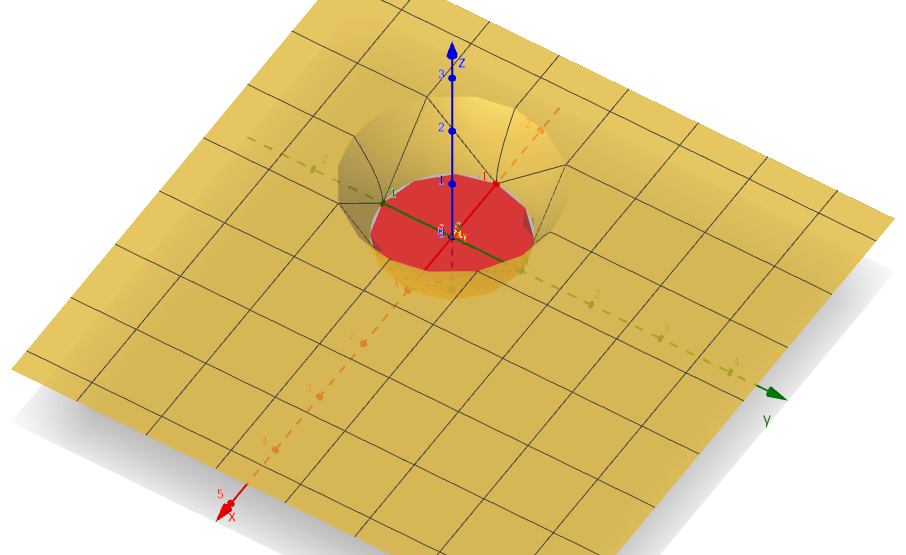
\includegraphics[scale=0.4]{../img/exercises/guide_02/08_a.png} 
\centering
\label{fig:2-8-a}
\end{figure}

Obsérvese la figura \ref{fig:2-8-a}. El gráfico de $f$ resulta la unión entre el plano $z=1$ (amarillo) y el plano $z=0$ (rojo), con agujeros de radio 2 y 1 respectivamente, unidos por una sección cónica (amarillo).

\subsection*{2.8.b}
\label{subsec:2.8.b}
\addcontentsline{toc}{subsection}{\nameref{subsec:2.8.b}}

Pensando de nuevo en términos de conjuntos de nivel, para $z = 0$ se tiene:

\begin{equation}
z = 0 \Rightarrow x^2 + y^2 = 1
\end{equation}

Para $z = 1$:

\begin{equation}
z = 1 \Rightarrow x^2 + \frac{y^2}{4} = 2 \Rightarrow \frac{x^2}{2} + \frac{y^2}{8} = 1
\end{equation}

Estos conjuntos de nivel no tienen puntos $(x,y)$ en común. La elipse de $z=1$ tiene semiejes $a = \sqrt{2} \approx 1,41$ y $b = \sqrt{8} \approx 2,82$, ambos mayores que el radio 1 de la circunferencia. Intuitivamente, existe al menos una superficie continua que une estas curvas. Teniendo en cuenta que la circunferencia es un caso particular de la elipse ($a=b$), se puede plantear los conjuntos de nivel de $f$ como elipses cuyos semiejes son funciones de $z$. 

\begin{equation}
\frac{x^2}{a(z)^2} + \frac{y^2}{b(z)^2} = 1
\end{equation}

Estas funciones $a(z)$ y $b(z)$ deben satisfacer:

\begin{subequations}
\begin{align}
& a(0) = 1 \\
& a(1) = \sqrt{2} \\
& b(0) = 1 \\
& b(1) = \sqrt{8}
\end{align}
\end{subequations}

Con dos pares de puntos para cada una, lo más directo es definirlas como funciones lineales:

\begin{subequations}
\begin{align}
& m_a = \frac{\sqrt{2}-1}{1-0} = \sqrt{2} - 1 \Rightarrow a(z) = (\sqrt{2}-1) z + 1 \\
& m_b = \frac{\sqrt{8}-1}{1-0} = \sqrt{8} - 1 \Rightarrow b(z) = (\sqrt{8}-1) z + 1
\end{align}
\end{subequations}

Dado que al reemplazar $a(z)$ y $b(z)$ resulta imposible despejar $z$ como función de $x$ e $y$, $f$ sólo puede ser definida de forma implícita. Para evitar problemas con los ceros de $a(z)$ y $b(z)$, se exige que $z$ sea mayor que el máximo de ambos, concretamente $z_1 = \frac{-1}{\sqrt{8}-1} \approx -0,546$.

\begin{equation}
\tcboxmath[colback=orange!25!white,colframe=orange,title=2.8.b]
{
\begin{array}{ll}
& F(x,y,z) = \frac{x^2}{[(\sqrt{2}-1)z+1]^2} + \frac{y^2}{[(\sqrt{8}-1)z+1]^2} - 1 \\
& Dom(F) = \{ (x, y, z) \in \Bbb R^3 / z > z_1 \} \\
& z = f(x,y) / \mathop{Graf}(f) = C_0(F) = \{ (x,y,z) \in \Bbb R^3 / F(x,y,z) = 0 \} 
\end{array}
}
\end{equation}

Sería adelantarse a los temas de la presente guía, pero siendo $F$ diferenciable, está garantizada la existencia de $f$ por el teorema de Cauchy-Dini. Por otro lado, el gráfico de $f$ es una especie de elipsoide cuyos semiejes crecen al crecer $z$, y decrecen al acercarse $z$ a $z_1$.

\subsection*{2.8.c}
\label{subsec:2.8.c}
\addcontentsline{toc}{subsection}{\nameref{subsec:2.8.c}}

El único conjunto de $\Bbb R^2$ donde $f$ no está definida es $x-y = 1$. Dado que las dos ramas que están definidas son continuas en todo $\Bbb R^2$, para que $f$ sea continua, ambas ramas deben tener el mismo valor punto a punto sobre $x-y = 1$. Evaluando dichas ramas en $x-y=1 \Leftrightarrow y = x-1$:

\begin{subequations}
\begin{align}
& \text{Rama } x-y<1:  x-y|_{y = x-1}= x-(x-1) = x - x + 1 = 1 \\
& \text{Rama } x-y>1:  (y-x)^2|_{y = x-1}= (x-1-x)^2 = (-1)^2 = 1
\end{align}
\end{subequations}

Las dos ramas valen, punto a punto, sobre la curva $x-y = 1$, la constante 1. Por lo tanto, $f$ es continua si se extiende cualquiera de las dos ramas al caso $x-y = 1$, o si se define que $f$ vale 1 sobre esa curva. Por ejemplo:

\begin{equation}
\tcboxmath[colback=orange!25!white,colframe=orange,title=2.8.c]
{
f(x,y) = \left\{ \begin{array}{ll}
x-y \text{ si } x-y \leq 1 \\
(y-x)^2 \text{ si } x-y > 1
\end{array} \right.
}
\end{equation}

\begin{figure}[ht]
\caption{\textbf{2-8-c}}
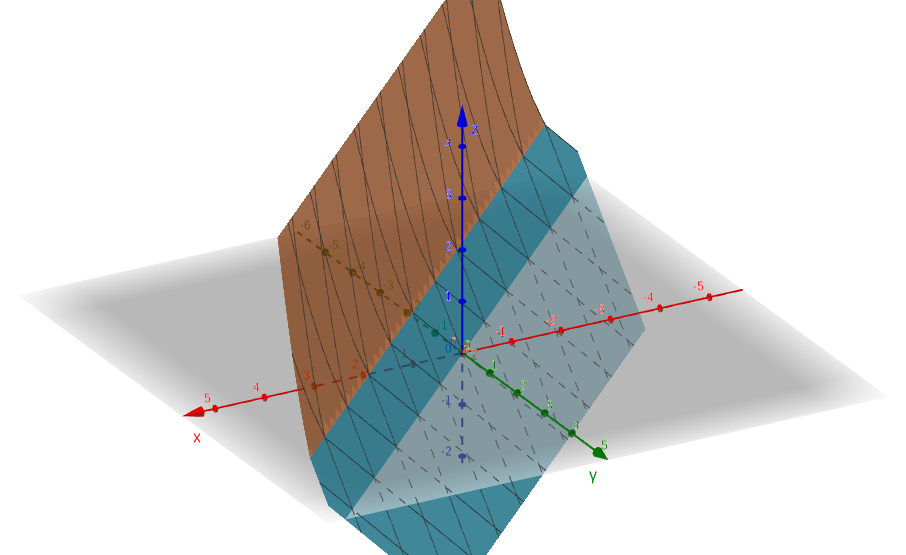
\includegraphics[scale=0.4]{../img/exercises/guide_02/08_c.png} 
\centering
\label{fig:2-8-c}
\end{figure}

Graficando $f$ definida de esta manera (ver figura \ref{fig:2-8-c}), se confirma su continuidad: es la unión de un semiplano (azul) y una sección de superficie cuadrática (naranja).

\section*{2.9}
\label{sec:2.9}
\addcontentsline{toc}{section}{\nameref{sec:2.9}}

\textbf{En los siguientes casos, calcular las derivadas parciales de $f$ en el punto indicado.}

\begin{enumerate}[(a)]
\bfseries

\item $f(x,y) = xy + x^2, P_0 = (2, 0)$

\item $f(x,y,z) = xz / (y+z), P_0 = (1, 1, 1)$

\item $f(x, y, z) = \ln(1 + e^{x+y^2 z}), P_0 = (0, 2, 0)$

\item $f(x,y) = \sin(x \sqrt{y}), P_0 = (\pi/3, 4)$

\item $f(x,y) = 1/\sqrt{x^2 + y^2}, P_0 = (-3, 4)$

\item $f(x,y) = \left\{ \begin{array}{ll}
\frac{2x^3 - y^3}{x^2 + 3y^2} \text{ si } (x,y) \neq (0,0) \\
0 \text{ si } (x,y) = (0,0)
\end{array} \right., P_0 = (0,0)$

\item $f(x,y) = \left\{ \begin{array}{ll}
\frac{x^2 - 2y^2}{x - y} \text{ si } (x,y) \neq (0,0) \\
0 \text{ si } (x,y) = (0,0)
\end{array} \right., P_0 = (0,0)$ 

\item $f(x,y) = \left\{ \begin{array}{ll}
0 \text{ si } xy \neq 0 \\
1 \text{ si } xy = 0
\end{array} \right., P_0 = (0,0)$

\item $f(x,y) = \int_{x}^{y^2} \sin(\ln(1 + t^3)) \mathop{dt}, P_0 = (1,2)$

\end{enumerate}

\subsection*{2.9.a}
\label{subsec:2.9.a}
\addcontentsline{toc}{subsection}{\nameref{subsec:2.9.a}}

Por definición, las derivadas parciales de un campo escalar de $n$ variables evaluadas en un punto son los siguientes límites, si existen:

\begin{equation}
\frac{\partial f}{\partial x_i}(P_0) = \lim_{h \rightarrow 0} \frac{f(P_0 + h e_i) - f(P_0)}{h}, e_i \in \Bbb R^n / e_j = 1 \text{ si } j = i, 0 \text{ en otro caso} 
\end{equation}

Aplicando a este caso:

\begin{subequations}
\begin{align}
& f(x,y) = xy + x^2, P_0 = (2,0) \\
& \frac{\partial f}{\partial x}(2,0) = \lim_{h \rightarrow 0} \frac{(2+h) 0 + (2+h)^2 - 4}{h} = \lim_{h \rightarrow 0} \frac{4 + 4h + h^2 - 4}{h} = \lim_{h \rightarrow 0} 4 + h = 4 \\
& \frac{\partial f}{\partial y}(2,0) = \lim_{h \rightarrow 0} \frac{2 (0+h) + 2^2 - 4}{h} = \lim_{h \rightarrow 0} \frac{2h}{h} = 2
\end{align}
\end{subequations}

Esto puede verificarse calculando las derivadas parciales de forma general y evaluando:

\begin{align}
& \frac{\partial f}{\partial x}(x,y) = y + 2x \Rightarrow \frac{\partial f}{\partial x}(2,0) = 4 \\
& \frac{\partial f}{\partial y}(x,y) = x \Rightarrow \frac{\partial f}{\partial y}(2,0) = 2
\end{align}

Para haber usado este segundo método de entrada, había que demostrar que el límite existe para todo $(x,y)$, o determinar para cuáles no existe. Por simplicidad, se utilizará el primer método para el resto del ejercicio.

\begin{equation}
\tcboxmath[colback=orange!25!white,colframe=orange,title=2.9.a]
{
\begin{array}{ll}
& \frac{\partial f}{\partial x}(2,0) = 4 \\
& \frac{\partial f}{\partial y}(2,0) = 2
\end{array}
}
\end{equation}

\subsection*{2.9.b}
\label{subsec:2.9.b}
\addcontentsline{toc}{subsection}{\nameref{subsec:2.9.b}}

Aplicando la definición:

\begin{subequations}
\begin{align}
& f(x,y,z) = \frac{xz}{y+z} \\
& \frac{\partial f}{\partial x}(1,1,1) = \lim_{h \rightarrow 0} \frac{1}{h} \left( \frac{(1+h)}{1+1} - \frac{1}{2} \right) = \lim_{h \rightarrow 0} \frac{1}{h} \left( \frac{1 + h - 1}{2} \right) = \frac{1}{2} \\
& \frac{\partial f}{\partial y}(1,1,1) = \lim_{h \rightarrow 0} \frac{1}{h} \left( \frac{1}{1+h+1} - \frac{1}{2} \right) = \lim_{h \rightarrow 0} \frac{1}{h} \left( \frac{2 - h - 2}{(h+2) 2} \right) = \lim_{h \rightarrow 0} \frac{-1}{(h+2)2} = -\frac{1}{4} \\
& \frac{\partial f}{\partial z}(1,1,1) = \lim_{h \rightarrow 0} \frac{1}{h} \left( \frac{1+h}{1+1+h} - \frac{1}{2} \right) = \lim_{h \rightarrow 0} \frac{1}{h} \left( \frac{2+2h-h-2}{(h+2) 2} \right) = \frac{1}{4}
\end{align}
\end{subequations}

\begin{equation}
\tcboxmath[colback=orange!25!white,colframe=orange,title=2.9.b]
{
\begin{array}{ll}
& \frac{\partial f}{\partial x}(1,1,1) = \frac{1}{2} \\
& \frac{\partial f}{\partial y}(1,1,1) = -\frac{1}{4} \\
& \frac{\partial f}{\partial z}(1,1,1) = \frac{1}{4}
\end{array}
}
\end{equation}

\subsection*{2.9.c}
\label{subsec:2.9.c}
\addcontentsline{toc}{subsection}{\nameref{subsec:2.9.c}}

Aplicando la definición:

\begin{subequations}
\begin{align}
& f(x, y, z) = \ln(1 + e^{x + y^2 z}), P_0 = (0, 2, 0) \Rightarrow f(P_0) = \ln(2) \\
& \frac{\partial f}{\partial x}(0, 2, 0) = \lim_{h \rightarrow 0} \frac{\ln(1+e^h) - \ln(2)}{h} \overset{L'H}{=} \lim_{h \rightarrow 0} \frac{\frac{1}{1+e^h} e^h}{1} = \frac{1}{2} \\
& \frac{\partial f}{\partial y}(0, 2, 0) = \lim_{h \rightarrow 0} \frac{\ln(1 + e^0)-\ln(2)}{h} = 0 \\
& \frac{\partial f}{\partial z}(0, 2, 0) = \lim_{h \rightarrow 0} \frac{\ln(1+e^{4h})-\ln(2)}{h} \overset{L'H}{=} \lim_{h \rightarrow 0} \frac{\frac{1}{1+e^{4h}} 4 e^{4h}}{1} = \frac{4}{2} = 2
\end{align}
\end{subequations}

Nótese que se aplicó la regla de L'Hôpital en algunas indeterminaciones del tipo $\frac{0}{0}$. Esto es válido porque los límites calculados son de una sola variable ($h$).

\begin{equation}
\tcboxmath[colback=orange!25!white,colframe=orange,title=2.9.c]
{
\begin{array}{ll}
& \frac{\partial f}{\partial x}(0, 2, 0) = \frac{1}{2} \\
& \frac{\partial f}{\partial y}(0, 2, 0) = 0 \\
& \frac{\partial f}{\partial z}(0, 2, 0) = 2
\end{array}
}
\end{equation}

\subsection*{2.9.d}
\label{subsec:2.9.d}
\addcontentsline{toc}{subsection}{\nameref{subsec:2.9.d}}

Aplicando la definición:

\begin{subequations}
\begin{align}
f(x, y) &= \sin(x \sqrt{y}), P_0 = \left( \frac{\pi}{3}, 4 \right) \Rightarrow f(P_0) = \frac{\sqrt{3}}{2} \\
\frac{\partial f}{\partial x}\left( \frac{\pi}{3}, 4 \right) &= \lim_{h \rightarrow 0} \frac{\sin\left[ \left( \frac{\pi}{3} + h \right) 2 \right] - \frac{\sqrt{3}}{2}}{h} \overset{L'H}{=} \lim_{h \rightarrow 0} \frac{\cos\left[ 2 \left(h + \frac{\pi}{3} \right) 2 \right]}{1} = 2 \cos\left( \frac{2}{3} \pi \right) = -1 & \\
\frac{\partial f}{\partial y}\left( \frac{\pi}{3}, 4 \right) &= \lim_{h \rightarrow 0} \frac{\sin\left( \frac{\pi}{3} \sqrt{4+h} \right) - \frac{\sqrt{3}}{2}}{h} \overset{L'H}{=} \lim_{h \rightarrow 0} = \lim_{h \rightarrow 0} \cos\left[ \frac{\pi}{3} (h+4)^{\frac{1}{2}} \right] \frac{d}{\mathop{dh}} \left[ \frac{\pi}{3} (h+4)^{\frac{1}{2}} \right] & \\
&= \lim_{h \rightarrow 0} \cos\left[ \frac{\pi}{3} (h+4)^{\frac{1}{2}} \right] \frac{\pi}{3} \frac{1}{2} (h+4)^{-\frac{1}{2}} = -\frac{\pi}{24}
\end{align}
\end{subequations}

\begin{equation}
\tcboxmath[colback=orange!25!white,colframe=orange,title=2.9.d]
{
\begin{array}{ll}
& \frac{\partial f}{\partial x}\left( \frac{\pi}{3}, 4 \right) = -1 \\
& \frac{\partial f}{\partial y}\left( \frac{\pi}{3}, 4 \right) = -\frac{\pi}{24}
\end{array}
}
\end{equation}

\subsection*{2.9.e}
\label{subsec:2.9.e}
\addcontentsline{toc}{subsection}{\nameref{subsec:2.9.e}}

Aplicando la definición:

\begin{subequations}
\begin{align}
& f(x, y) = (x^2 + y^2)^{-\frac{1}{2}}, P_0 = (-3, 4) \Rightarrow f(P_0) = \frac{1}{5} \\
& \frac{\partial f}{\partial x}(-3, 4) = \lim_{h \rightarrow 0} \frac{[(-3+h)^2 + 16]^{-\frac{1}{2}} - \frac{1}{5} } {h} \overset{L'H}{=} \lim_{h \rightarrow 0} -\frac{1}{2} [(h-3)^2 + 16]^{-\frac{3}{2}} 2 (h-3) = 3 \cdot 25^{-\frac{3}{2}} \\
& \frac{\partial f}{\partial y}(-3, 4) = \lim_{h \rightarrow 0} \frac{[9 + (4+h)^2]^{-\frac{1}{2}} - \frac{1}{5} } {h} \overset{L'H}{=} \lim_{h \rightarrow 0} -\frac{1}{2} [(h+4)^2 + 9]^{-\frac{3}{2}} 2 (h+4) = -4 \cdot 25^{-\frac{3}{2}}
\end{align}
\end{subequations}

\begin{equation}
\tcboxmath[colback=orange!25!white,colframe=orange,title=2.9.e]
{
\begin{array}{ll}
& \frac{\partial f}{\partial x}(-3, 4) = 3 \cdot 25^{-\frac{3}{2}} = 0,024 \\
& \frac{\partial f}{\partial y}(-3, 4) = -4 \cdot 25^{-\frac{3}{2}} = -0,032
\end{array}
}
\end{equation}

\subsection*{2.9.f}
\label{subsec:2.9.f}
\addcontentsline{toc}{subsection}{\nameref{subsec:2.9.f}}

Aplicando la definición:

\begin{subequations}
\begin{align}
& f(x, y) = \left\{ \begin{array}{ll}
\frac{2x^3 - y^3}{x^2 + 3y^2} \text{ si } (x,y) \neq (0,0) \\
0 \text{ si } (x,y) = (0,0)
\end{array} \right., P_0 = (0, 0) \Rightarrow f(P_0) = 0 \\
& \frac{\partial f}{\partial x}(0, 0) = \lim_{h \rightarrow 0} \frac{f(0+h, 0)-f(0)}{h} = \lim_{h \rightarrow 0} \frac{1}{h} \frac{2h^3}{h^2} = \lim_{h \rightarrow 0} \frac{2h}{h} = 2 \\
& \frac{\partial f}{\partial y}(0, 0) = \lim_{h \rightarrow 0} \frac{f(0, 0+h)-f(0)}{h} = \lim_{h \rightarrow 0} \frac{1}{h} \frac{-h^3}{3h^2} = \lim_{h \rightarrow 0} \frac{1}{h} \left(-\frac{1}{3}h\right) = -\frac{1}{3}
\end{align}
\end{subequations}

\begin{equation}
\tcboxmath[colback=orange!25!white,colframe=orange,title=2.9.f]
{
\begin{array}{ll}
& \frac{\partial f}{\partial x}(0, 0) = 2 \\
& \frac{\partial f}{\partial y}(0, 0) = -\frac{1}{3}
\end{array}
}
\end{equation}

\subsection*{2.9.g}
\label{subsec:2.9.g}
\addcontentsline{toc}{subsection}{\nameref{subsec:2.9.g}}

Aplicando la definición:

\begin{subequations}
\begin{align}
& f(x, y) = \left\{ \begin{array}{ll}
\frac{x^2 - 2y^2}{x - y} \text{ si } (x,y) \neq (0,0) \\
0 \text{ si } (x,y) = (0,0)
\end{array} \right., P_0 = (0, 0) \Rightarrow f(P_0) = 0 \\
& \frac{\partial f}{\partial x}(0, 0) = \lim_{h \rightarrow 0} \frac{f(0+h, 0)-f(0)}{h} = \lim_{h \rightarrow 0} \frac{1}{h} \frac{h^2}{h} = 1 \\
& \frac{\partial f}{\partial y}(0, 0) = \lim_{h \rightarrow 0} \frac{f(0, 0+h)-f(0)}{h} = \lim_{h \rightarrow 0} \frac{1}{h} \frac{-2h^2}{-h} = 2
\end{align}
\end{subequations}

\begin{equation}
\tcboxmath[colback=orange!25!white,colframe=orange,title=2.9.g]
{
\begin{array}{ll}
& \frac{\partial f}{\partial x}(0, 0) = 1 \\
& \frac{\partial f}{\partial y}(0, 0) = 2
\end{array}
}
\end{equation}

\subsection*{2.9.h}
\label{subsec:2.9.h}
\addcontentsline{toc}{subsection}{\nameref{subsec:2.9.h}}

Aplicando la definición:

\begin{subequations}
\begin{align}
& f(x, y) = \left\{ \begin{array}{ll}
0 \text{ si } xy \neq 0 \\
1 \text{ si } xy = 0
\end{array} \right., P_0 = (0, 0) \Rightarrow f(P_0) = 1 \\
& \frac{\partial f}{\partial x}(0, 0) = \lim_{h \rightarrow 0} \frac{f(0+h, 0)-f(0)}{h} = \lim_{h \rightarrow 0} \frac{1-1}{h} = 0 \\
& \frac{\partial f}{\partial y}(0, 0) = \lim_{h \rightarrow 0} \frac{f(0, 0+h)-f(0)}{h} = \lim_{h \rightarrow 0} \frac{1-1}{h} = 0
\end{align}
\end{subequations}

A priori, se podría pensar que $f$ es discontinua en $(0,0)$, pero no lo es, al menos en las direcciones de los ejes. La función $f$ vale 1 en el origen y a lo largo de los ejes $x$ e $y$, en donde $x$, $y$ o ambos son nulos.

\begin{equation}
\tcboxmath[colback=orange!25!white,colframe=orange,title=2.9.h]
{
\begin{array}{ll}
& \frac{\partial f}{\partial x}(0, 0) = 0 \\
& \frac{\partial f}{\partial y}(0, 0) = 0
\end{array}
}
\end{equation}

\subsection*{2.9.i}
\label{subsec:2.9.i}
\addcontentsline{toc}{subsection}{\nameref{subsec:2.9.i}}

\begin{equation}
f(x, y) = \int_{x}^{y^2} \sin [ \ln ( 1 + t^3 ) ] \mathop{dt}, P_0 = (1, 2)
\end{equation}

El integrando puede no estar definido para ciertos valores de $t$. Específicamente, el argumento del logaritmo debe ser mayor a cero.

\begin{equation}
1 + t^3 > 0 \Rightarrow t^3 > -1 \Rightarrow t > -1
\end{equation}

Los argumentos de $f$ son los límites de integración; considerando el dominio del integrando, $y$ está elevado al cuadrado y por ende siempre es positivo. En cambio, $x$ debe ser mayor a -1. Ergo:

\begin{equation}
\mathop{Dom}(f) = \{ (x,y) \in \Bbb R^2 / x > -1 \}
\end{equation}

El punto $P_0$ pertenece entonces al dominio de $f$. Al intentar evaluar $f(P_0)$, se concluye que la primitiva del integrando no es trivial, y un cálculo numérico determina que $f(1,2) = K_0 \approx 0,64960$. Aplicando entonces la definición para las derivadas parciales:

\begin{equation}
\frac{\partial f}{\partial x}(1,2) = \lim_{h \rightarrow 0} \frac{ \int_{1+h}^4 \sin[ \ln(1 + t^3) ] \mathop{dt} - f(1,2) }{h} 
\end{equation}

Antes de aplicar la regla de L'Hopital a la indeterminación $\frac{0}{0}$, considérese, por el Teorema Fundamental del Cálculo:

\begin{subequations}
\begin{align}
& g(t) = \sin[ \ln(1 + t^3) ] \text{ es acotada en el intervalo } [1,4] \Rightarrow \\
& \int_a^t g(\tau) \mathop{d\tau} = G(t) + C \\
& G'(t) = g(t)
\end{align}
\end{subequations}

Siendo $g$ continua en $[1,4]$, vale entonces la regla de Barrow. Aplicando LHôpital, y recordando que se deriva respecto a la variable $h$:

\begin{subequations}
\begin{align}
\frac{\partial f}{\partial x}(1,2) &= \lim_{h \rightarrow 0} \frac{G(4) - G(1+h) - K_0}{h} & \\
&= \lim_{h \rightarrow 0} \frac{-G'(1+h) (1+h)'}{1} = -G'(1) = -g(1) = \sin( \ln 2 ) \approx 0,63896
\end{align}
\end{subequations}

La misma idea sirve para calcular la derivada parcial en $y$:

\begin{subequations}
\begin{align}
\frac{\partial f}{\partial x}(1,2) &= \lim_{h \rightarrow 0} \frac{ \int_{1}^{(2+h)^2} \sin[ \ln(1 + t^3) ] \mathop{dt} - K_0 }{h} = \lim_{h \rightarrow 0} \frac{G[(h+2)^2] - G(1) - K_0}{h} & \\
&= \lim_{h \rightarrow 0} G'[(h+2)^2] 2 (h+2) = 4 G'(4) = 4 g(4) = 4 \sin( \ln 65 ) \approx -3.4349
\end{align}
\end{subequations}

\begin{equation}
\tcboxmath[colback=orange!25!white,colframe=orange,title=2.9.i]
{
\begin{array}{ll}
& \frac{\partial f}{\partial x}(1, 2) = \sin( \ln 2 ) \approx 0,63896 \\
& \frac{\partial f}{\partial y}(1, 2) = 4 \sin( \ln 65 ) \approx -3.4349
\end{array}
}
\end{equation}

\section*{2.10}
\label{sec:2.10}
\addcontentsline{toc}{section}{\nameref{sec:2.10}}

\textbf{Hallar las derivadas de de segundo orden de:}

\begin{enumerate}[(a)]
\bfseries

\item $\arctan \left( \frac{x}{y} \right)$

\item $\sqrt{\frac{x^2}{a^2} + \frac{y^2}{b^2}}$

\item $\ln(x^2 + y)$

\end{enumerate}

\subsection*{2.10.a}
\label{subsec:2.10.a}
\addcontentsline{toc}{subsection}{\nameref{subsec:2.10.a}}

\begin{equation}
f(x,y) = \arctan \left( \frac{x}{y} \right)
\end{equation}

La función arco tangente, como función de una variable, es derivable, y su derivada $\left( \frac{1}{1+x^2} \right)$ también. Por ende, se espera que existan las derivadas parciales de primer y segundo orden, y se calculan de forma directa. Las derivadas de primer orden resultan entonces:

\begin{subequations}
\begin{align}
& f_x(x,y) = \frac{\partial}{\partial x} \left[ \arctan \left( \frac{x}{y} \right) \right] = \frac{1}{1 + \left( \frac{x}{y} \right)^2} \frac{1}{y} = \frac{1}{ \left( 1 + \frac{x^2}{y^2} \right) y } = \frac{1}{y + \frac{x^2}{y}} \\
& f_y(x,y) = \frac{\partial}{\partial y} \left[ \arctan \left( x y^{-1} \right) \right] = \frac{1}{1 + \left( \frac{x}{y} \right)^2 } \cdot x \cdot (-1) \cdot y^{-2} = \frac{-x}{x^2 + y^2}
\end{align}
\end{subequations}

Y las de segundo orden:

\begin{subequations}
\begin{align}
f_{xy}(x,y) &= \frac{\partial}{\partial y} \left[ (y + x^2 y^{-1})^{-1} \right] = (-1) (y + x^2 y^{-1})^{-2} [1 + x^2 (-1) y^{-2}] & \\
&= (-1) \frac{1}{(y + \frac{x^2}{y})^2} \left( 1 - \frac{x^2}{y^2} \right) = \frac{\frac{x^2}{y^2} - 1}{ \left( \frac{x^2}{y} + y \right) \left( \frac{x^2}{y} + y \right) } \frac{y^2}{y^2} & \\
&= \tcboxmath[colback=orange!25!white,colframe=orange,title=$f_{xy}$]{ \frac{x^2 - y^2}{(x^2 + y^2)^2} } & \\
f_{yx}(x,y) &= \frac{\partial}{\partial x} \left[ (-x) (x^2 + y^2)^{-1} \right] = (-1) (x^2 + y^2)^{-1} + (-x) (-1) (x^2 + y^2)^{-2} 2x & \\
&= \frac{-1}{x^2 + y^2} + \frac{2x^2}{ (x^2 + y^2)^2 } = \frac{(-1)(x^2 + y^2) + 2x^2}{(x^2 + y^2)^2} & \\
&= \tcboxmath[colback=orange!25!white,colframe=orange,title=$f_{yx}$]{ \frac{x^2 - y^2}{(x^2 + y^2)^2} } & \\
f_{xx}(x,y) &= \frac{\partial}{\partial x} \left[ \left( \frac{1}{y} x^2 + y \right)^{-1} \right] = (-1) \left( \frac{1}{y} x^2 + y \right)^{-2} \frac{1}{y} 2x = \frac{-2x}{\left( \frac{x^2}{y} + y \right)^2} & \\
&= \frac{-2x}{ \left( \frac{x^2}{y} + y \right) \left( \frac{x^2}{y} + y \right) } \frac{y^2}{y^2} \\
&= \tcboxmath[colback=orange!25!white,colframe=orange,title=$f_{xx}$]{ \frac{-2xy^2}{(x^2 + y^2)^2} } & \\
f_{yy}(x,y) &= \frac{\partial}{\partial y} \left[ -x (y^2 + x^2)^{-1}  \right] = (-x) (-1) (y^2 + x^2)^{-2} 2y & \\
&= \tcboxmath[colback=orange!25!white,colframe=orange,title=$f_{yy}$]{ \frac{2xy}{(x^2 + y^2)^2} }
\end{align}
\end{subequations}

Nótese que $f_{xy}(x,y) = f_{yx}(x,y)$, lo cual era de esperarse por el Teorema de Schwartz.

\subsection*{2.10.b}
\label{subsec:2.10.b}
\addcontentsline{toc}{subsection}{\nameref{subsec:2.10.b}}

\begin{equation}
f(x,y) = \left( \frac{x^2}{a^2} + \frac{y^2}{b^2} \right)^{\frac{1}{2}}
\end{equation}

En este caso, no hay problemas de continuidad. Utilizando el mismo enfoque del inciso anterior, las derivadas de primer orden son:

\begin{subequations}
\begin{align}
& f_x(x,y) = \frac{\partial}{\partial x} \left[ \left( \frac{x^2}{a^2} + \frac{y^2}{b^2} \right)^\frac{1}{2} \right] = \frac{1}{2} \left( \frac{x^2}{y^2} + \frac{y^2}{b^2} \right)^{-\frac{1}{2}} \frac{1}{a^2} 2x = \frac{x}{a^2} \left( \frac{x^2}{a^2} + \frac{y^2}{b^2} \right)^{-\frac{1}{2}} \\
& f_y(x,y) = \frac{\partial}{\partial y} \left[ \left( \frac{y^2}{b^2} + \frac{x^2}{a^2} \right)^\frac{1}{2} \right] = \frac{1}{2} \left( \frac{y^2}{b^2} + \frac{x^2}{a^2} \right)^{-\frac{1}{2}} \frac{1}{b^2} 2y = \frac{y}{b^2} \left( \frac{x^2}{a^2} + \frac{y^2}{b^2} \right)^{-\frac{1}{2}}
\end{align}
\end{subequations}

Y las de segundo orden:

\begin{subequations}
\begin{align}
f_{xy}(x,y) &= \frac{\partial}{\partial y} \left[ \frac{x}{a^2} \left( \frac{y^2}{b^2} + \frac{x^2}{a^2} \right)^{-\frac{1}{2}} \right] = \frac{x}{a^2} \frac{-1}{2} \left( \frac{x^2}{a^2} + \frac{y^2}{b^2}\right)^{-\frac{3}{2}} \frac{2y}{b^2} & \\
&= \tcboxmath[colback=orange!25!white,colframe=orange,title=$f_{xy}$]{ \frac{-xy}{(ab)^2} \left( \frac{x^2}{a^2} + \frac{y^2}{b^2} \right)^{-\frac{3}{2}} } & \\
f_{yx}(x,y) &= \frac{\partial}{\partial x} \left[ \frac{y}{b^2} \left( \frac{x^2}{a^2} + \frac{y^2}{b^2} \right)^{-\frac{1}{2}} \right] = \frac{y}{b^2} \frac{-1}{2} \left( \frac{x^2}{a^2} + \frac{y^2}{b^2}\right)^{-\frac{3}{2}} \frac{2x}{a^2} & \\
&= \tcboxmath[colback=orange!25!white,colframe=orange,title=$f_{yx}$]{ \frac{-xy}{(ab)^2} \left( \frac{x^2}{a^2} + \frac{y^2}{b^2} \right)^{-\frac{3}{2}} } & \\
f_{xx}(x,y) &= \frac{\partial}{\partial x} \left[ \frac{x}{a^2} \left( \frac{x^2}{a^2} + \frac{y^2}{b^2} \right)^{-\frac{1}{2}} \right] = \frac{1}{a^2} \left( \frac{x^2}{a^2} + \frac{y^2}{b^2} \right)^{-\frac{1}{2}} + \frac{x}{a^2} \frac{-1}{2} \left( \frac{x^2}{a^2} + \frac{y^2}{b^2} \right)^{-\frac{3}{2}} \frac{2x}{a^2} & \\
&= \tcboxmath[colback=orange!25!white,colframe=orange,title=$f_{xx}$]{ \frac{1}{a^2} \left( \frac{x^2}{a^2} + \frac{y^2}{b^2} \right)^{-\frac{1}{2}} - \frac{x^2}{a^2} \left( \frac{x^2}{a^2} + \frac{y^2}{b^2} \right)^{-\frac{3}{2}} } & \\
f_{yy}(x,y) &= \frac{\partial}{\partial y} \left[ \frac{y}{b^2} \left( \frac{x^2}{a^2} + \frac{y^2}{b^2} \right)^{-\frac{1}{2}} \right] = \frac{1}{b^2} \left( \frac{x^2}{a^2} + \frac{y^2}{b^2} \right)^{-\frac{1}{2}} + \frac{y}{b^2} \frac{-1}{2} \left( \frac{x^2}{a^2} + \frac{y^2}{b^2} \right)^{-\frac{3}{2}} \frac{2y}{b^2} & \\
&= \tcboxmath[colback=orange!25!white,colframe=orange,title=$f_{yy}$]{ \frac{1}{b^2} \left( \frac{x^2}{a^2} + \frac{y^2}{b^2} \right)^{-\frac{1}{2}} - \frac{y^2}{b^2} \left( \frac{x^2}{a^2} + \frac{y^2}{b^2} \right)^{-\frac{3}{2}} }
\end{align}
\end{subequations}

\subsection*{2.10.c}
\label{subsec:2.10.c}
\addcontentsline{toc}{subsection}{\nameref{subsec:2.10.c}}

El dominio de $f$ debe satisfacer:

\begin{equation}
x^2 + y > 0 \Rightarrow y > -x^2 \Rightarrow
\end{equation}

Con eso en mente, las derivadas de primer orden son:

\begin{subequations}
\begin{align}
& f_x(x,y) = \frac{\partial}{\partial x} \left[ \ln(x^2 + y) \right] = \frac{1}{x^2 + y} 2x = \frac{2x}{x^2 + y} \\
& f_y(x,y) = \frac{\partial}{\partial y} \left[ \ln(y + x^2) \right] = \frac{1}{y + x^2} 1 = \frac{1}{x^2 + y}
\end{align}
\end{subequations}

Y las de segundo orden son:

\begin{subequations}
\begin{align}
f_{xy}(x,y) &= \frac{\partial}{\partial y} \left[ 2x (y + x^2)^{-1} \right] = 2x (-1) (y + x^2)^{-2} \\
&= \tcboxmath[colback=orange!25!white,colframe=orange,title=$f_{xy}$]{ \frac{-2x}{(x^2 + y^2)^2} } & \\
f_{yx}(x,y) &= \frac{\partial}{\partial x} \left[ (x^2 + y)^{-1} \right] = (-1) (x^2 + y)^{-2} 2x \\
&= \tcboxmath[colback=orange!25!white,colframe=orange,title=$f_{yx}$]{ \frac{-2x}{(x^2 + y^2)^2} } & \\
f_{xx}(x,y) &= \frac{\partial}{\partial x} \left[ 2x (x^2 + y)^{-1} \right] = 2 (x^2 + y)^{-1} + 2x (-1) (x^2 + y)^{-2} 2x & \\
&= \frac{2}{x^2 + y} - \frac{4x^2}{(x^2 + y)^2} = \frac{2 (x^2 + y)-4x^2}{(x^2 + y)^2} & \\
&= \tcboxmath[colback=orange!25!white,colframe=orange,title=$f_{xx}$]{ \frac{-2x^2 + y}{(x^2 + y)^2} } & \\
f_{yy}(x,y) &= \frac{\partial}{\partial y} \left[ (y + x^2)^{-1} \right] = (-1) (y + x^2)^{-2} & \\
&= \tcboxmath[colback=orange!25!white,colframe=orange,title=$f_{yy}$]{ \frac{-1}{(x^2 + y)^2} }
\end{align}
\end{subequations}

\section*{2.11}
\label{sec:2.11}
\addcontentsline{toc}{section}{\nameref{sec:2.11}}

\textbf{Sea:}

\begin{equation}
f(x,y) = \left\{ \begin{array}{ll}
xy \frac{x^2 - y^2}{x^2 + y^2} \text{ si } (x,y) \neq (0,0) \\
0 \text{ si } (x,y) = (0,0)
\end{array} \right.
\end{equation}

\textbf{Mostrar que las derivadas cruzadas en $(0,0)$ de $f$ existen y son distintas. ¿Es $C^2$ la función f?}

El primer paso sería calcular las derivadas primeras. Fuera del punto problemático que representa el origen, $f$ es continua y derivable. Por lo tanto, para $(x,y) \neq 0$:

\begin{subequations}
\begin{align}
f_x(x,y) &= \frac{\partial}{\partial x} \left[ xy \frac{x^2 - y^2}{x^2 + y^2} \right] = \frac{\partial}{\partial x} \left[ \frac{x^3y - xy^3}{x^2 + y^2} \right] \\
f_y(x,y) &= \frac{\partial}{\partial y} \left[ \frac{x^3y - xy^3}{x^2 + y^2} \right]
\end{align}
\end{subequations}

Recuérdese la regla del cociente para derivadas de una variable, que puede aplicarse al calcular derivadas parciales:

\begin{equation}
\left( \frac{u}{v} \right)' = \frac{u'v - uv'}{v^2}
\end{equation}

Aplicando esta regla primero para $f_x$:

\begin{subequations}
\begin{align}
u &= x^3 y - xy^3 \Rightarrow u_x = y 3x^2 - y^3 = 3x^2y - y^3 \\
v &= x^2 + y^2 \Rightarrow v_x = 2x \\
f_x(x,y) &= \frac{(3x^2y - y^3)(x^2 + y^2) - (x^3y - xy^3) 2x}{(x^2 + y^2)^2} \\
&= \frac{3x^4y + 3x^2y^3-x^2y^3-y^5-2x^4y+2x^2y^3}{(x^2 + y^2)^2} \\
&= \frac{x^4y+4x^2y^3-y^5}{(x^2 + y^2)^2}
\end{align}
\end{subequations}

Esta expresión vale para todo par $(x,y)$ excepto $(0,0)$. Analizando dicho punto con la definición:

\begin{equation}
f_x(0,0) = \lim_{h \rightarrow 0} \frac{f(0+h, 0) - f(0,0)}{h} = \lim_{h \rightarrow 0} \frac{1}{h} \left[ (0+h) 0 \frac{h^2 - 0^2}{h^2 + 0^2} \right] = 0
\end{equation}


Por ende, la expresión completa de la derivada primera respecto a $x$ es:

\begin{equation}
f_x(x,y) = \left\{ \begin{array}{ll}
\frac{x^4y+4x^2y^3-y^5}{(x^2 + y^2)^2} \text{ si } (x,y) \neq (0,0) \\
0 \text{ si } (x,y) = (0,0)
\end{array} \right.
\end{equation}

Calculando $f_y$ de la misma manera:

\begin{subequations}
\begin{align}
u &= x^3 y - xy^3 \Rightarrow u_y = x^3 - 3xy^2 \\
v &= x^2 + y^2 \Rightarrow v_y = 2y \\
f_y(x,y) &= \frac{(x^3 - 3xy^2)(x^2 + y^2)-(x^3y - xy^3)2y}{(x^2 + y^2)^2} \\
&= \frac{x^5 +x^3y^2 -3x^3y^2-3xy^4-2x^3y^2+2xy^4}{(x^2 + y^2)^2} \\
&= \frac{x^5 - 4x^3y^2 -xy^4}{(x^2 + y^2)^2}
\end{align}
\end{subequations}

\begin{equation}
f_y(0,0) = \lim_{h \rightarrow 0} \frac{f(0, 0+h) - f(0,0)}{h} = \lim_{h \rightarrow 0} \frac{1}{h} \left[ 0 (0+h) \frac{0^2 - h^2}{0^2 + h^2} \right] = 0
\end{equation}

La expresión completa de la derivada primera respecto a $y$ es:

\begin{equation}
f_y(x,y) = \left\{ \begin{array}{ll}
\frac{x^5 - 4x^3y^2 -xy^4}{(x^2 + y^2)^2} \text{ si } (x,y) \neq (0,0) \\
0 \text{ si } (x,y) = (0,0)
\end{array} \right.
\end{equation}

Con las expresiones completas de $f_x$ y $f_y$, es posible calcular las derivadas cruzadas en el origen utilizando la definición:

\begin{subequations}
\begin{align}
f_{xy}(0,0) &= \lim_{h \rightarrow 0} \frac{f_x(0, 0+h) - f_x(0,0)}{h} = \lim_{h \rightarrow 0} \frac{1}{h} \left[ \frac{0^4 h + 4 0^2 h^3 - h^5}{(0^2 + h^2)^2} \right] = \lim_{h \rightarrow 0} \frac{-h^5}{h^5} = -1 \\
f_{yx}(0,0) &= \lim_{h \rightarrow 0} \frac{f_y(0+h, 0) - f_y(0,0)}{h} = \lim_{h \rightarrow 0} \frac{1}{h} \left[ \frac{h^5 - 4 h^3 0^2 - h 0^4}{(h^2 + 0^2)^2} \right] = \lim_{h \rightarrow 0} \frac{h^5}{h^5} = 1
\end{align}
\end{subequations}

Esto prueba que las derivadas cruzadas no coinciden en el origen. Por el teorema de Schwartz, si $f \in C^2$, $fxy$ y $fyx$ deben ser iguales punto a punto. Dado que esto no se cumple en el origen, necesariamente $f \notin C^2$.

\section*{2.12}
\label{sec:2.12}
\addcontentsline{toc}{section}{\nameref{sec:2.12}}

\textbf{Analizar la existencia de las derivadas direccionales en el origen de las siguientes funciones, y calcularlas:}

\begin{enumerate}[(a)]
\bfseries

\item $f(x,y) = \left\{ \begin{array}{ll}
x^2 - y &\text{ si } x > |y| \\
x - y &\text{ si } x \leq |y|
\end{array} \right.$

\item $f(x,y) = \left\{ \begin{array}{ll}
x^2 + y &\text{ si } x > 2y \\
3 &\text{ si } x \leq 2y
\end{array} \right.$

\item $f(x,y,z) = \left\{ \begin{array}{ll}
x+y+z &\text{ si } z^2 > x^2 + y^2 \wedge z > 0 \\
0 &\text{ en otros casos }
\end{array} \right.$

\end{enumerate}

\subsection*{2.12.a}
\label{subsec:2.12.a}
\addcontentsline{toc}{subsection}{\nameref{subsec:2.12.a}}

Por definición, la derivada direccional en el punto $P_0$ es:

\begin{equation}
f'(P_0, \overrightarrow{v}) = \lim_{h \rightarrow 0} \frac{f(P_0 + h \overrightarrow{v}) - f(P_0)}{h}
\end{equation}

En este caso, $P_0 = (0,0) \Rightarrow f(P_0) = f(0,0) = 0 - 0 = 0$ (porque $0 \leq |0|$: el origen está en la segunda rama).

Planteando el vector $\overrightarrow{v}$ en sus componentes: $\overrightarrow{v} = (v_x, v_y)$:

\begin{subequations}
\begin{align}
f'(P_0, \overrightarrow{v}) &= \lim_{h \rightarrow 0} \frac{f((0,0) + h (v_x, v_y)) - f(0,0)}{h} \\
&= \lim_{h \rightarrow 0} \frac{f(h v_x, h v_y)}{h}
\end{align}
\end{subequations}

Caso I: $h v_x > |h v_y| \Leftrightarrow \frac{h}{|h|} v_x > |v_y| \overset{h > 0}{\Leftrightarrow} v_x > |v_y|$

\begin{equation}
f'(P_0, \overrightarrow{v}) = \lim_{h \rightarrow 0} \frac{h^2 {v_x}^2 - h v_y}{h} = \lim_{h \rightarrow 0} h v_x - v_y = -v_y
\end{equation}

Caso II: $h v_x \leq |h v_y| \Leftrightarrow v_x \leq |v_y|$

\begin{equation}
f'(P_0, \overrightarrow{v}) = \lim_{h \rightarrow 0} \frac{h v_x - h v_y}{h} = v_x -v_y
\end{equation}

Finalmente:

\begin{equation}
\tcboxmath[colback=orange!25!white,colframe=orange,title=2.11.a]
{
f'((0,0), (v_x, v_y)) = \left\{ \begin{array}{ll}
-v_y &\text{ si } v_x > |v_y| \\
v_x - v_y &\text{ si } v_x \leq |v_y|
\end{array} \right.
}
\end{equation}

\subsection*{2.12.b}
\label{subsec:2.12.b}
\addcontentsline{toc}{subsection}{\nameref{subsec:2.12.b}}

Por definición:

\begin{equation}
f'(P_0, \overrightarrow{v}) = \lim_{h \rightarrow 0} \frac{f(h v_x, h v_y)-f(0,0)}{h} = \lim_{h \rightarrow 0} \frac{f(h v_x, h v_y)-3}{h}
\end{equation}

Caso I: $h v_x > 2 h v_y \Leftrightarrow v_x > 2 v_y$

\begin{equation}
f'(P_0, \overrightarrow{v}) = \lim_{h \rightarrow 0} \frac{h^2{v_x}^2 + h v_y -3}{h} = \frac{-3}{0} = \nexists
\end{equation}

Caso II: $h v_x \leq 2 h v_y \Leftrightarrow v_x \leq 2 v_y$

\begin{equation}
f'(P_0, \overrightarrow{v}) = \lim_{h \rightarrow 0} \frac{3 -3}{h} = 0
\end{equation}

Finalmente:

\begin{equation}
\tcboxmath[colback=orange!25!white,colframe=orange,title=2.12.b]
{
f'((0,0), (v_x, v_y)) = \left\{ \begin{array}{ll}
\nexists &\text{ si } v_x > 2 v_y \\
0 &\text{ si } v_x \leq 2 v_y
\end{array} \right.
}
\end{equation}

\subsection*{2.12.c}
\label{subsec:2.12.c}
\addcontentsline{toc}{subsection}{\nameref{subsec:2.12.c}}

Por definición:

\begin{equation}
f'(P_0, \overrightarrow{v}) = \lim_{h \rightarrow 0} \frac{f(h v_x, h v_y, h v_z)-f(0,0,0)}{h} = \lim_{h \rightarrow 0} \frac{f(h v_x, h v_y, h v_z)}{h}
\end{equation}

Caso I: $(h v_z)^2 > (h v_x)^2 + (h v_y)^2 \wedge h v_z > 0 \overset{h >0}{\Leftrightarrow} v_z^2 > v_x^2 + v_y^2 \wedge v_z > 0$

\begin{equation}
f'(P_0, \overrightarrow{v}) = \lim_{h \rightarrow 0} \frac{h v_x + h v_y + h v_z}{h} = v_x + v_y + v_z
\end{equation}

Caso II: otros casos

\begin{equation}
f'(P_0, \overrightarrow{v}) = \lim_{h \rightarrow 0} \frac{0}{h} = 0
\end{equation}

Finalmente:

\begin{equation}
\tcboxmath[colback=orange!25!white,colframe=orange,title=2.12.c]
{
f'((0,0,0), (v_x, v_y, v_z)) = \left\{ \begin{array}{ll}
v_x + v_y + v_z &\text{ si } v_z^2 > v_x^2 + v_y^2 \wedge v_z > 0 \\
0 &\text{ en otros casos }
\end{array} \right.
}
\end{equation}

\section*{2.13}
\label{sec:2.13}
\addcontentsline{toc}{section}{\nameref{sec:2.13}}

\textbf{Sea $C$ la curva dada por $\sigma(t) = (R \cos(t), R\sin(t)), t \in [0, 2\pi)$. Hallar la ecuación de su recta tangente en $t = \pi/4$.}

Para una curva monoparamétrica como $\sigma$, la derivada componente a componente $\sigma'(t)$ representa el vector dirección de la recta tangente en el punto $\sigma(t)$. Para este caso, dado que ambas componentes son funciones derivables por ser seno y coseno, resulta:

\begin{equation}
\sigma'(t) = (-R \sin(t), R \cos(t)) \Rightarrow \sigma'\left( \frac{\pi}{4} \right) = \left( \frac{-\sqrt{2}}{2} R, \frac{\sqrt{2}}{2} R \right)
\end{equation}

Entonces, la ecuación vectorial de la recta tangente es:

\begin{equation}
L_T : \sigma'(\pi/4) t + P_0
\end{equation}

El punto $P_0$ es un punto cualquiera por el que pasa la recta. Se sabe que pasa por $\sigma(\pi/4) = (\sqrt{2}/2 R, \sqrt{2}/2 R)$. Ergo:

\begin{subequations}
\begin{align}
L_T &: \left( \frac{-\sqrt{2}}{2} R, \frac{\sqrt{2}}{2} R \right) t + \left( \frac{\sqrt{2}}{2} R, \frac{\sqrt{2}}{2} R \right) \\
x &= \frac{-\sqrt{2}}{2} R t + \frac{\sqrt{2}}{2} R \\
y &= \frac{\sqrt{2}}{2} R t + \frac{\sqrt{2}}{2} R
\end{align}
\end{subequations}

Sumando $x$ e $y$ miembro a miembro, se obtiene la ecuación clásica de la recta:

\begin{equation}
x + y = \sqrt{2} R
\end{equation}

\begin{equation}
\tcboxmath[colback=orange!25!white,colframe=orange,title=2.13]
{
y = -x + \sqrt{2} R
}
\end{equation}

Este resultado concuerda con que $\sigma$ es una circunferencia de radio $R$, y $t = \pi/4$ corresponde al punto asociado al ángulo $\pi/4$. La recta tangente tiene pendiente $-1$, lo cual corresponde a un ángulo de $-pi/4$. Geométricamente, tiene sentido.

\section*{2.14}
\label{sec:2.14}
\addcontentsline{toc}{section}{\nameref{sec:2.14}}

\textbf{Sea $C$ la curva dada por $\sigma(t) = (t^2, t^3 + 1, t^3-1), t \in [0, 4]$. Hallar la ecuación de su recta tangente y su plano normal en $t = 2$.}

\subsection*{2.14.a}
\label{subsec:2.14.a}
\addcontentsline{toc}{subsection}{\nameref{subsec:2.14.a}}

El punto correspondiente a $t = 2$ es:

\begin{equation}
\sigma(2) = (2^2, 2^3+1, 2^3-1) = (4, 9, 7)
\end{equation}

El vector tangente en $t = 2$ es:

\begin{equation}
\sigma'(t) = (2t, 3t^2, 3t^2) \Rightarrow \sigma'(2) = (2 \cdot 2, 3 \cdot 4, 3 \cdot 4) = (4, 12, 12)
\end{equation}

El vector tangente es el vector dirección de la recta tangente; con un punto por donde pase, queda determinada la ecuación vectorial de la recta tangente:

\begin{equation}
\tcboxmath[colback=orange!25!white,colframe=orange,title=2.14.a]
{
L_T : (4, 12, 12) t + (4, 9, 7)
}
\end{equation}

El vector tangente es ortogonal al plano normal; por ende, su normal coincide con el vector tangente. Y dado que el punto $\sigma(2)$ pertenece al plano, satisface su ecuación y eso determina el parámetro $D$ faltante:

\begin{subequations}
\begin{align}
& 4 (x - 4) + 12 (y - 9) + 12 (z - 7) = 0 \\
& 4x - 16 + 12y - 108 + 12z - 84 = 0 \\
& x + 3y +3z - 52 = 0
\end{align}
\end{subequations}

\begin{equation}
\tcboxmath[colback=orange!25!white,colframe=orange,title=2.14.a]
{
\Pi_N : x + 3y + 3z - 52 = 0
}
\end{equation}

\subsection*{2.14.b}
\label{subsec:2.14.b}
\addcontentsline{toc}{subsection}{\nameref{subsec:2.14.b}}

Dado que tres puntos en $\Bbb R^3$ determinan un plano, tomando 3 puntos arbitrarios de la curva se obtiene:

\begin{subequations}
\begin{align}
& P = \sigma(0) = (0, 1, -1) \\
& Q = \sigma(1) = (1, 2, 0) \\
& R = \sigma(2) = (4, 9, 7) \\
& \overrightarrow{N} = \overrightarrow{PQ} \times \overrightarrow{QR} = (Q-P) \times (R-Q) = (1, 1, 1) \times (3, 7, 7) = (0, -4, 4)
\end{align}
\end{subequations}

Conocido $\overrightarrow{N}$, se puede obtener la ecuación del plano evaluando un punto conocido, por ejemplo $P$:

\begin{subequations}
\begin{align}
& 0 (x-0) -4 (y-1) + 4 (z+1) = 0 \\
& -4y +4 + 4z + 4 = 0 \\
& -y + 1 + z + 1 = 0
& \Pi: -y + z + 2 = 0
\end{align}
\end{subequations}

Ahora bien, para que la curva $C$ sea plana, sus puntos deben pertenecer al plano $\Pi$ para todo valor de $t$ en el intervalo $[0,4]$:

\begin{subequations}
\begin{align}
& -y(t) + z(t) + 2 = 0 \\
& -t^3-1 +t^3-1 + 2 = 0\\
0 = 0
\end{align}
\end{subequations}

Dado que $\sigma(t)$ satisface la ecuación del plano $\Pi$ para todo valor de $t$, la curva completa está contenida en el plano, o en otras palabras, es plana.

\subsection*{2.14.c}
\label{subsec:2.14.c}
\addcontentsline{toc}{subsection}{\nameref{subsec:2.14.c}}

La intersección entre la curva y el plano puede conceptualizarse como los puntos de la curva que satisfacen la ecuación del plano. En términos de $t$:

\begin{equation}
y(t) + z(t) = 2 \Rightarrow t^3 +1 +t^3 -1 = 2 \Rightarrow 2t^3 = 2 \Rightarrow t = 1
\end{equation}

La intersección resulta entonces un único punto $P$:

\begin{equation}
\tcboxmath[colback=orange!25!white,colframe=orange,title=2.14.c]
{
P = \sigma(1) = (1, 2, 0)
}
\end{equation}

\section*{2.15}
\label{sec:2.15}
\addcontentsline{toc}{section}{\nameref{sec:2.15}}

\textbf{En los siguientes casos, hallar una parametrización de la curva definida por el par de ecuaciones, y calcular su recta tangente en el punto indicado.}

\begin{enumerate}[(a)]
\bfseries

\item $x^2 + y^2 + z^2 = 2, z = \sqrt{x^2 + y^2}, P_0 = (0, 1, 1)$

\item $z = x + y^2, x = y^2, P_0 = (4, 2, 8)$

\item $x^2 + y^2 + z^2 = 6, z = x^2 + y^2, P_0 = (1, 1, 2)$

\end{enumerate}

\subsection*{2.15.a}
\label{subsec:2.15.a}
\addcontentsline{toc}{subsection}{\nameref{subsec:2.15.a}}

Elevando la segunda ecuación al cuadrado miembro a miembro:

\begin{equation}
z^2 = (\sqrt{ x^2+y^2 })^2
\end{equation}

Dado que el radicando es siempre mayor o igual que cero por ser la suma de dos cuadrados, no es necesario aplicar módulo al cancelar la raíz y el cuadrado en el lado derecho.

\begin{equation}
z^2 = x^2 + y^2
\end{equation}

Reemplazando en la primera ecuación:

\begin{equation}
x^2 + y^2 + (x^2 + y^2) = 2 \Rightarrow 2x^2 + 2y^2 = 2 \Rightarrow x^2 + y^2 = 1
\end{equation}

Dado que $z = \sqrt{x^2 + y^2}$, resulta $z = \sqrt{1} = 1$. Por lo tanto, la curva a parametrizar es un círculo unitario en el plazo $z=1$. Una parametrización posible es:

\begin{equation}
\tcboxmath[colback=orange!25!white,colframe=orange,title=2.15.a]
{
\sigma(t) = (\cos(t), \sin(t), 1), t \in [0, 2\pi)
}
\end{equation}

Para calcular la recta tangente en $P_0$ es necesario hallar el valor del parámetro $t$ asociado a $P_0$; llámese $t_0$.

\begin{equation}
\sigma(t_0) = P_0 \Rightarrow (\cos(t_0), \sin(t_0), 1) = (0, 1, 1) \Rightarrow t_0 = \frac{\pi}{2}
\end{equation}

Conocido $t_0$, puede obtenerse el vector dirección de la recta tangente evaluando $\sigma'(t_0)$:

\begin{equation}
\sigma'(t) = (-\sin(t), \cos(t), 0) \Rightarrow \sigma'(t_0) = (-1, 0, 0)
\end{equation}

Resulta entonces la recta tangente en $P_0$:

\begin{equation}
\tcboxmath[colback=orange!25!white,colframe=orange,title=2.15.a]
{
L_T: (-1, 0, 0) \alpha + (0, 1, 1)
}
\end{equation}

\subsection*{2.15.b}
\label{subsec:2.15.b}
\addcontentsline{toc}{subsection}{\nameref{subsec:2.15.b}}

La segunda ecuación pone $x$ en función de $y$ al establecer que $x = y^2$. Reemplazando eso en la primera ecuación, resulta $z = y^2 + y^2 = 2y^2$. Dado que $x$ y $z$ dependen sólo de $y$, $y$ puede hacer las veces de parámetro:

\begin{equation}
\tcboxmath[colback=orange!25!white,colframe=orange,title=2.15.b]
{
\sigma(t) = (t^2, t, 2t^2), t \in \Bbb R
}
\end{equation}

Para hallar la recta tangente en $P_0$, es necesario hallar el valor $t_0$ que satisfaga $\sigma(t_0) = P_0$.

\begin{equation}
(t_0^2, t_0, 2t_0^2) = (4, 2, 8) \Rightarrow t_0 = 2
\end{equation}

Conocido $t_0$, puede obtenerse el vector dirección de la recta tangente evaluando $\sigma'(t_0)$:

\begin{equation}
\sigma'(t) = (2t, 1, 4t) \Rightarrow \sigma'(t_0) = (4, 1, 8)
\end{equation}

Resulta entonces la recta tangente en $P_0$:

\begin{equation}
\tcboxmath[colback=orange!25!white,colframe=orange,title=2.15.b]
{
L_T: (4, 1, 8) \alpha + (4, 2, 8)
}
\end{equation}

\subsection*{2.15.c}
\label{subsec:2.15.c}
\addcontentsline{toc}{subsection}{\nameref{subsec:2.15.c}}

La segunda ecuación establece que $z = x^2 + y^2$. Reemplazando $x^2 + y^2$ por $z$ en la primera ecuación, se obtiene una ecuación cuadrática en $z$.

\begin{equation}
\underbrace{x^2 + y^2}_{z} + z^2 = 6 \Rightarrow z + z^2 = 6 \Rightarrow z^2 + z - 6 = 0 \Rightarrow z = 2 \vee z = -3
\end{equation}

Dado que $z = x^2 + y^2$, queda descartada la solución $z = -3$. Por ende, $z = 2$, y $x^2 + y^2 = 2$. La curva es un círculo de radio $\sqrt{2}$ en el plano $z = 2$.

\begin{equation}
\tcboxmath[colback=orange!25!white,colframe=orange,title=2.15.c]
{
\sigma(t) = (\sqrt{2} \cos(t), \sqrt{2} \sin(t), 2), t \in [0, 2\pi)
}
\end{equation}

Para hallar la recta tangente en $P_0$, es necesario hallar el valor $t_0$ que satisfaga $\sigma(t_0) = P_0$.

\begin{equation}
(\sqrt{2} \cos(t_0), \sqrt{2} \sin(t_0), 2) = (1, 1, 2) \Rightarrow t_0 = \frac{\pi}{4}
\end{equation}

Conocido $t_0$, puede obtenerse el vector dirección de la recta tangente evaluando $\sigma'(t_0)$:

\begin{equation}
\sigma'(t) = (-\sqrt{2} \sin(t_0), \sqrt{2} \cos(t_0), 0) \Rightarrow \sigma'(t_0) = (-1, 1, 0)
\end{equation}

Resulta entonces la recta tangente en $P_0$:

\begin{equation}
\tcboxmath[colback=orange!25!white,colframe=orange,title=2.15.c]
{
L_T: (-1, 1, 0) \alpha + (1, 1, 2)
}
\end{equation}

\section*{2.16}
\label{sec:2.16}
\addcontentsline{toc}{section}{\nameref{sec:2.16}}

\textbf{Resolver los siguientes problemas:}

\begin{enumerate}[(a)]
\bfseries

\item Una abeja vuela ascendiendo a lo largo de la curva intersección de $z = x^4 + xy^3 + 12$ con $x = 1$. En el punto $(1, -2, 5)$ sigue a lo largo de la tangente. ¿Dónde cruza la abeja el plano $y = 1$?

\item Una partícula se mueve en el plano de manera que su posición al tiempo $t$ es $r(t) = (t - \sin(t), 1 - \cos(t))$. Hallar los máximos de los módulos de su velocidad y su aceleración. Dibujar aproximadamente la trayectoria y los vectores velocidad y aceleración.

\item Una partícula se mueve a lo largo de la parte superior de la parábola de ecuación $y^2 = 2x$ de izquierda a derecha con rapidez de 5 unidades por segundo. ¿Cuál es su vector velocidad al pasar por $(2,2)$?

\end{enumerate}

\subsection*{2.16.a}
\label{subsec:2.16.a}
\addcontentsline{toc}{subsection}{\nameref{subsec:2.16.a}}

La trayectoria puede considerarse un sistema de ecuaciones:

\begin{equation}
\left\{ \begin{array}{ll}
z = x^4 + xy^3 + 12 \\
x = 1
\end{array} \right.
\end{equation}

Reemplazando la segunda ecuación en la primera, resulta:

\begin{equation}
z = 1 + y^3 + 12 \Rightarrow z = y^3 + 13
\end{equation}

La coordenada $x$ está fija en 1, la coordenada $y$ está libre, y la coordenada $z$ depende de la coordenada $y$. Entonces, puede parametrizarse la trayectoria según:

\begin{equation}
r(t) = (1, t, t^3 + 13)
\end{equation}

Para analizar la tangente en el punto $(1, -2, 5)$ es necesario saber a qué valor $t_0$ corresponde.

\begin{equation}
(1, t_0, t_0^3+13) = (1, -2, 5) \Rightarrow t_0 = -2
\end{equation}

Conocido $t_0$, puede evaluarse el vector tangente en dicho punto a través de $r'(t)$.

\begin{equation}
r'(t) = (0, 1, 3t^2) \Rightarrow r'(t_0) = (0, 1, 12)
\end{equation}

La recta tangente en $(1, -2, 5)$ es entonces:

\begin{equation}
L_T: (0, 1, 12) \alpha + (1, 2, -5)
\end{equation}

Para calcular la intersección de esta recta con el plano $y = 1$, basta con igualar su coordenada $y$ a 1 y calcular $\alpha_0$:

\begin{equation}
(x(\alpha), y(\alpha), z(\alpha)) = (1, \alpha+2, 12\alpha-5)
\end{equation}

Si $y(\alpha) = 1 \Rightarrow 1 = \alpha + 2 \Rightarrow \alpha = -1$; reemplazando dicho valor de $\alpha$ en las otras coordenadas, se obtiene el punto intersección buscado:

\begin{equation}
\tcboxmath[colback=orange!25!white,colframe=orange,title=2.16.a]
{
Q = (1, 1, -17)
}
\end{equation}

\subsection*{2.16.b}
\label{subsec:2.16.b}
\addcontentsline{toc}{subsection}{\nameref{subsec:2.16.b}}

La velocidad es la derivada primera de la trayectoria, y la aceleración es la derivada segunda. Ergo:

\begin{subequations}
\begin{align}
r(t) &= (t - \sin(t), 1 - \cos()t) \\
v(t) &= r'(t) = (1 - \cos(t), \sin(t)) \\
a(t) &= r''(t) = v'(t) = (\sin(t), \cos(t))
\end{align}
\end{subequations}

El módulo de la velocidad es entonces la siguiente función del tiempo:

\begin{equation}
||v(t)|| = \sqrt{(1-\cos(t))^2 + \sin^2(t)}
\end{equation}

Maximizar la raíz equivale a maximizar el radicando, por lo tanto maximizar $||v(t)||$ equivale a maximizar:

\begin{equation}
f(t) = (1- \cos(t))^2 + \sin^2(t)
\end{equation}

Expandiendo el binomio:

\begin{subequations}
\begin{align}
f(t) &= 1 - 2\cos(t) + \underbrace{\cos^2(t) + \sin^2(t)}_{1} \\
&= 2 - 2 \cos(t) \\
f'(t) &= 2 \sin(t) \\
f''(t) &= 2 \cos(t)
\end{align}
\end{subequations}

Los ceros de $f'(t)$ son $t_k = k\pi, k \in \Bbb Z$. Para ver qué tipo de extremo son, es necesario evaluar $f''(t_k)$. Recuérdese que si $f'(t_i) = 0 \wedge f''(t_i) < 0$, entonces en $t_i$ hay un máximo local; si es mayor a cero, es un mínimo local, y si es cero, no se sabe (se requiere más información).

\begin{equation}
f''(t_k) = 2 \cos(k\pi) = \left\{ \begin{array}{ll}
1 \text{ si } k \text{ es par} \\
-1 \text{ si } k \text{ es impar}
\end{array} \right.
\end{equation}

El vector velocidad es máximo en los puntos:

\begin{equation}
\tcboxmath[colback=orange!25!white,colframe=orange,title=2.16.b]
{
t_k = (2k+1) \pi, k \in \Bbb Z
}
\end{equation}

En cuanto a la aceleración, $||a(t)|| = \sqrt{\sin^2(t) + \cos^2(t)} = 1$.

\begin{equation}
\tcboxmath[colback=orange!25!white,colframe=orange,title=2.16.b]
{
||a(t)|| = \mathop{cte} = 1
}
\end{equation}

Para graficar, obsérvese que todas las expresiones tienen senos y cosenos de período $2\pi$; por ende, se elige $\pi/2$ como incremento para las tablas de valores.

\begin{center}
\begin{tabular}{||c c c c||} 
 \hline
 t & r(t) & v(t) & a(t) \\ [0.5ex] 
 \hline\hline
 0 & (0,0) & (0,0) & (1,0) \\ 
 \hline
 $\pi/2$ & (0.6, 1.0) & (1,1) & (1,0) \\
 \hline
 $\pi$ & (3.1, 2.0) & (2,0) & (0,-1) \\
 \hline
 $3 \pi/2$ & (5.7, 1) & (1,-1) & (-1,0) \\
 \hline
 $2 \pi$ & (6.3, 0) & (0,0) & (0,1) \\
 \hline
 $5 \pi/2$ & (6.8, 1) & (1,1) & (1,0) \\
 \hline
 $3 \pi$ & (9.4, 2) & (2,0) & (0,-1) \\ [1ex] 
 \hline
\end{tabular}
\end{center}

Se observa que lo único que no es $2\pi$-periódico es la componente $x$ de $r(t)$, por su término lineal. Pero todo lo demás se repite cada $2\pi$. Gráficamente:

\begin{figure}[ht]
\caption{Trayectoria, velocidad y aceleración}
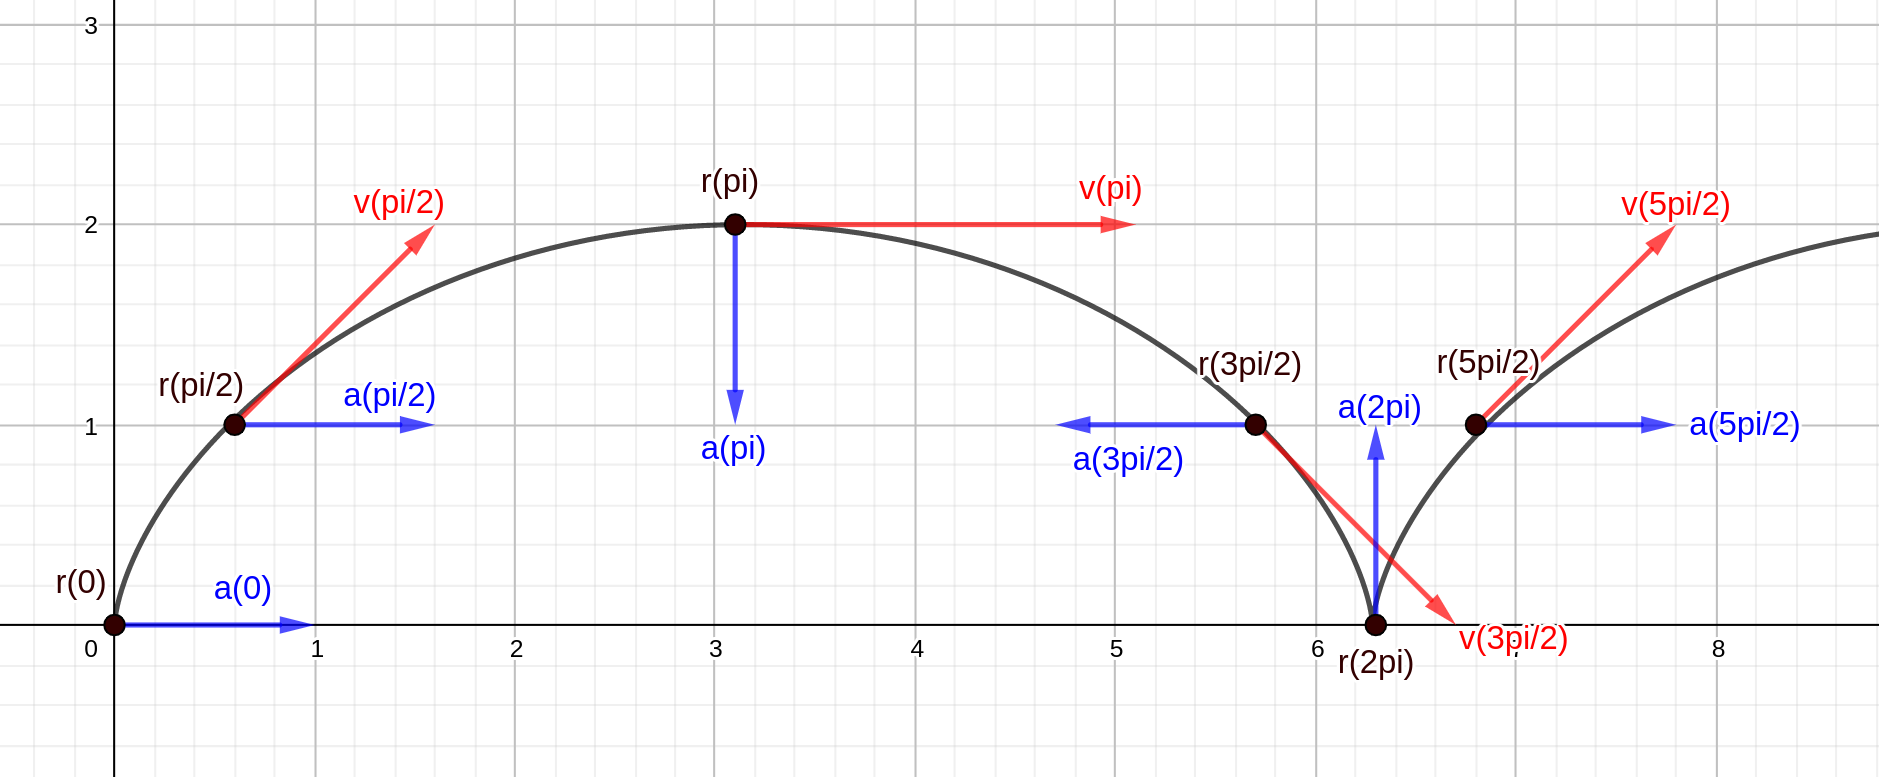
\includegraphics[scale=1]{../img/exercises/guide_02/16_b.png} 
\centering
\label{fig:2-16-b}
\end{figure}

\subsection*{2.16.c}
\label{subsec:2.16.c}
\addcontentsline{toc}{subsection}{\nameref{subsec:2.16.c}}

La distancia recorrida sobre la curva desde $t=a$ (posición inicial) al tiempo $t$ (posición final), llámese $s(t)$, puede calcularse como:

\begin{equation}
s(t) = \int_{a}^t ||r'(\tau)|| \mathop{d\tau}
\end{equation}

En esta expresión, $r(t) = (x(t), y(t))$ es la trayectoria. No tiene que ser necesariamente bidimensional; esto vale para $\Bbb R^n$. Para el caso particular en que la velocidad es de módulo constante, la distancia es el producto del módulo de la velocidad por el tiempo: $s(t) = v t$. Expandiendo la norma de $r'(t)$, resulta:

\begin{equation}
s(t) = v t = \int_{a}^t \sqrt{ \left( \frac{\mathop{dx}}{\mathop{d\tau}} \right)^2 + \left( \frac{\mathop{dy}}{\mathop{d\tau}} \right)^2 } \mathop{d\tau}
\end{equation}

Para el caso en que una coordenada es función de la otra, esta expresión puede simplificarse. Por ejemplo, si $y = f(x)$, por la regla de la cadena resulta:

\begin{equation}
v t = \int_{a}^t \sqrt{ \left( \frac{\mathop{dx}}{\mathop{d\tau}} \right)^2 + \left( \frac{\mathop{df}}{\mathop{dx}} \frac{\mathop{dx}}{\mathop{d\tau}} \right)^2 } \mathop{d\tau}
\end{equation}

Sacando factor común $\left( \frac{\mathop{dx}}{\mathop{d\tau}} \right)^2$:

\begin{equation}
v t = \int_{a}^t \sqrt{ \left( \frac{\mathop{dx}}{\mathop{d\tau}} \right)^2 \left[ 1 + \left( \frac{\mathop{df}}{\mathop{dx}} \right)^2\right] } \mathop{d\tau}
\end{equation}

El factor $\left[ 1 + \left( \frac{\mathop{df}}{\mathop{dx}} \right)^2\right]$ no depende de la variable de integración $\tau$, por lo tanto puede salir de la integral:

\begin{subequations}
\begin{align}
v t &= \sqrt{ \left[ 1 + \left( \frac{\mathop{df}}{\mathop{dx}} \right)^2\right] } \int_{a}^t \sqrt{ \left( \frac{\mathop{dx}}{\mathop{d\tau}} \right)^2 } \mathop{d\tau} \\
&= \sqrt{ \left[ 1 + \left( \frac{\mathop{df}}{\mathop{dx}} \right)^2\right] } \int_{a}^t \frac{\mathop{dx}}{\mathop{d\tau}} \mathop{d\tau}
\end{align}
\end{subequations}

Sin perder de vista que $x$ es una función del tiempo, la integral de $\frac{\mathop{dx}}{\mathop{d\tau}}$ es $x(\tau)$, por lo cual:

\begin{equation}
v t = \sqrt{ \left[ 1 + \left( \frac{\mathop{df}}{\mathop{dx}} \right)^2\right] } (x(t) - x(a))
\end{equation}

Cambiando la notación $x(t)$ a $x$, sin perder de vista que es una función del tiempo, y asumiendo $x(a) = 0$ para simplificar, resulta:

\begin{equation}
v t = \sqrt{ 1 + [f'(x)]^2 } x
\end{equation}

Si en esta expresión se puede despejar algebraicamente $x$ como función de $t$, luego es trivial hallar $y(t) = f(x(t))$. Con ello se obtiene una expresión cerrada para $r(t)$. Puede ocurrir que no haya solución cerrada para $x(t)$ o la coordenada elegida. Si con todas las coordenadas ocurre lo mismo, sólo queda como opción resolver numéricamente.

Para este caso particular, $v = 5$, y $2x = y^2 \Rightarrow y = \sqrt{2} x^{\frac{1}{2}}$. No se toma módulo para $y$ porque el enunciado dice que se recorre la rama superior, que corresponde a $y > 0$. Resulta entonces la relación $y = f(x)$ para este caso:

\begin{align}
y = f(x) = \sqrt{2} x^{\frac{1}{2}} \Rightarrow f'(x) = \sqrt{2} \frac{1}{2} x^{-\frac{1}{2}} = \frac{\sqrt{2}}{2} x^{-\frac{1}{2}}
\end{align}

Reemplazando:

\begin{subequations}
\begin{align}
5t &= \sqrt{1 + \left( \frac{\sqrt{2}}{2} x^{-\frac{1}{2}} \right)^2} x \\
5t &= \sqrt{1 + \frac{1}{2} x^{-1}} x
\end{align}
\end{subequations}

Elevando al cuadrado miembro a miembro (no se toma módulo porque al estar en la parte superior de la curva, $x > 0$ y por ende el radicando también es positivo):

\begin{subequations}
\begin{align}
25t^2 &= \left(1 + \frac{1}{2} x^{-1} \right) x^2 \\
25t^2 &= x^2 + \frac{1}{2} x \\
0 &= x^2 + \frac{1}{2} x - 25t^2
\end{align}
\end{subequations}

Resulta una ecuación cuadrática con $a = 1$, $b = \frac{1}{2}$ y $c = -25t^2$. El discriminante es:

\begin{equation}
\Delta = b^2 - 4ac = \frac{1}{4} - 4 (-25 t^2) = \frac{1 + 400 t^2}{4} > 0
\end{equation}

Hay dos soluciones posibles, pero sólo una cumple $x(t) \geq 0 \forall t \geq 0$, y es la que suma la raíz del discriminante.

\begin{subequations}
\begin{align}
x &= \frac{1}{2} (-b + \sqrt{\Delta}) = \frac{1}{2} \left( -\frac{1}{2} + \frac{\sqrt{400t^2 + 1}}{2} \right) \\
x(t) &= \frac{1}{4} (400t^2 + 1)^\frac{1}{2} - \frac{1}{4}
\end{align}
\end{subequations}

Conocido $x(t)$, puede obtenerse $y(t) = \sqrt{2} \sqrt{x}$:

\begin{equation}
y(t) = \sqrt{2} \left[ \frac{1}{4} (400t^2 + 1)^\frac{1}{2} - \frac{1}{4} \right]^\frac{1}{2}
\end{equation}

Antes de continuar, vale la pena calcular las derivadas $x'(t)$ e $y'(t)$ para verificar si satisfacen que $||r'(t)|| = ||(x'(t), y'(t))|| = 5$. Aplicando la regla de la cadena:

\begin{subequations}
\begin{align}
x'(t) &= \frac{1}{4} \frac{1}{2} (400t^2 + 1)^{-\frac{1}{2}} 800t \\
&= 100t (400t^2 + 1)^{-\frac{1}{2}} \\
y'(t) &= \sqrt{2} \frac{1}{2} x(t)^{-\frac{1}{2}} x'(t) \\
&= \sqrt{2} \frac{1}{2} \left[ \frac{1}{4} (400t^2 + 1)^{\frac{1}{2}} - \frac{1}{4} \right]^{-\frac{1}{2}} 100t (400t^2 + 1)^{-\frac{1}{2}} \\
&= 50 \sqrt{2} t \left\{ \left[ \frac{1}{4} (400t^2 + 1)^{\frac{1}{2}} - \frac{1}{4} \right] (400t^2 + 1) \right\}^{-\frac{1}{2}} \\
&= 100 \sqrt{2} t \left[ (400t^2 + 1)^{\frac{3}{2}} - (400t^2 + 1) \right]^{-\frac{1}{2}}
\end{align}
\end{subequations}

Es muy engorroso demostrar algebraicamente que $x'(t)^2 + y'(t)^2 = 25 \forall t > 0$, pero numéricamente se verifica, con Octave por ejemplo.

Verificados $x(t)$ e $y(t)$, el próximo paso es hallar el valor $t_0$ que satisface $r(t_0) = (2, 2)$. Siendo más sencilla la expresión de $x(t)$, se calcula a través de ella y se verifica con $y(t)$.

\begin{align}
2 &= \frac{1}{4} (400 t_0^2 + 1)^{\frac{1}{2}} - \frac{1}{4} \\
\frac{9}{4} &= \frac{1}{4} (400 t_0^2 + 1)^{\frac{1}{2}} \\
9^2 &= 400 t_0^2 + 1 \\
\frac{81-1}{400} &= t_0^2 \\
\frac{1}{5} &= t_0^2 \\
\sqrt{\frac{1}{5}} &= t_0 = \frac{\sqrt{5}}{5}
\end{align}

Se omite la verificación de $y(t_0) = 2$ por brevedad, pero se cumple. Finalmente, el vector velocidad en el punto $(2,2)$ es simplemente $r'(t_0)$:

\begin{equation}
\tcboxmath[colback=orange!25!white,colframe=orange,title=2.16.c]
{
v(t_0) = r'(t_0) \approx (4.9690, 2.4845)
}
\end{equation}

La norma de este vector es aproximadamente $5.5$, en lugar de 5 como cabría esperar. A esta altura no se supone que se manejen conceptos de análisis numérico, pero las expresiones de $x'(t)$ e $y'(t)$ son numéricamente inestables para valores pequeños como $t_0$, por contener restas de números similares y potencias. Eso causa la discrepancia en la norma y podría paliarse re-escribiendo las cuentas para evaluarlas de manera que no propaguen tanto el error de redondeo, pero eso excede los contenidos de esta materia. El concepto importante de este ejercicio es la aplicación de la regla de la cadena para simplificar el cálculo de la distancia recorrida sobre la curva; si sólo se planteara que $r'(t)$ tiene norma constante igual a 5 y la relación entre $x(t)$ e $y(t)$ dada por la curva, se llegaría a una ecuación diferencial no lineal sin solución cerrada.

\end{document}
